\documentclass[a4paper,11pt,table,dvipsnames]{article}

% Fonts and symbols
\usepackage{lmodern}
\usepackage{amsmath,amssymb}
\usepackage[utf8]{inputenc}
\usepackage[T1]{fontenc}
\usepackage{inconsolata}
\usepackage{wasysym}
\usepackage{microtype}

% Layout, page setup
\usepackage[margin=2.5cm,a4paper]{geometry}
\usepackage{titlesec}
\usepackage{appendix}
\usepackage{multicol}
\usepackage{multirow}
\usepackage{parskip}
\usepackage{tabto}
\usepackage{pdflscape}
\usepackage{enumitem}
\usepackage{adjustbox}
\usepackage[super]{nth}

% Science and language typesetting
\usepackage{bm}
\usepackage{physics}
\usepackage[
  arc-separator = \,,
  retain-explicit-plus,
  inter-unit-product = \cdot,
  detect-weight=true,
  detect-family=true,
  range-phrase=--,
  range-units=single
]{siunitx}
\usepackage[version=4]{mhchem}
\usepackage{nicematrix}
\usepackage[makeroom]{cancel}
\usepackage{circledsteps}
\usepackage[british]{babel}
\usepackage{csquotes}

% Graphics, captions, tables
\usepackage{graphicx}
\usepackage{float}
\usepackage{tikz,tikz-3dplot}
\usepackage{pgfplots}
\usepackage{pdfpages}
\usepackage[justification=centering, labelfont={small,bf}, font={small}]{caption}
\usepackage{subcaption}
\usepackage{array}
\usepackage{tabularx}
\usepackage{booktabs}
\usepackage[outline]{contour}

% TikZ options setup
\usetikzlibrary{
  calc,
  arrows,
  arrows.meta,
  positioning,
  decorations.pathreplacing,
  decorations.markings,
  decorations.text,
  calligraphy,
  pgfplots.dateplot,
  shapes.geometric
}

% References and links
\usepackage{hyperref}
\usepackage[noabbrev]{cleveref}
\usepackage[nottoc,numbib]{tocbibind}

% Miscellaneous
\usepackage{datetime2}
\usepackage{iftex,etoolbox,expl3,xparse}

\pgfplotsset{compat=1.18}
\AtBeginDocument{\RenewCommandCopy\qty\SI}

% ---------------------------------------------------------------------------

\title{Implementazione Client BLE}
\author{Andrea Zorzi -- BillyApp}
\date{Versione 1.0.0 \\ \today}

\begin{document}

\maketitle

\tableofcontents

\newpage

\section{Scopo e perimetro}

Questo documento descrive l'implementazione lato client del modello BLE definito in \emph{Architettura BLE lato Client e Server}.

\begin{itemize}
    \item piattaforme: iOS ed Android;
    \item strato condiviso: Kotlin Multiplatform Mobile (KMM);
    \item BLE e UI: implementate in modo nativo per ogni piattaforma.
\end{itemize}

\subsection{Perimetro}
Questo documento si concentra sull'implementazione del client BLE, escludendo la parte backend e le funzionalità di UI.
Argomenti trattati:
\begin{itemize}
    \item logica di advertising, scanning e lettura dei dati;
    \item gestione locale dell'identificativo \(B_{\text{id}}\);
    \item integrazione con KMM per le API condivise;
    \item gestione errori e permessi.
\end{itemize}

Sono esclusi:
\begin{itemize}
    \item architettura ed implementazione lato backend;
    \item dettagli del modello crittografico e rotazione chiavi AES;
\end{itemize}

\section{Panoramica architetturale}
L'architettura del client BLE si basa su una separazione tra logica condivisa e implementazioni specifiche per piattaforma.

\paragraph{UI}
La UI è implementata in modo nativo per ogni piattaforma:
\begin{itemize}
    \item schermate, view-model, state management;
    \item stato dell'applicazione ed interazioni utente.
\end{itemize}

\paragraph{BLE}
La logica BLE è implementata in modo nativo per ogni piattaforma, e si occupa di:
\begin{itemize}
    \item advertising di \(B_{\text{id}}\);
    \item scanning e parsing dei pacchetti \(B_{\text{id}}\);
    \item gestione ruoli: peripheral e central;
    \item monitoraggio stato Bluetooth, permessi e background modes.
\end{itemize}

\paragraph{KMM}
Il modulo KMM gestisce lo strato condiviso tra le piattaforme, e si occupa di:
\begin{itemize}
    \item contratti API;
    \item client HTTP;
    \item repository condivisi per la persistenza locale.
\end{itemize}

\subsection{Principi di progettazione}
L'architettura del client BLE segue i seguenti principi di progettazione:
\begin{itemize}
    \item \textbf{Separation of Concerns}: separazione chiara tra logica BLE, UI e strato condiviso;
    \item \textbf{Modularità}: componenti indipendenti e riutilizzabili;
    \item \textbf{Testabilità}: progettazione per facilitare i test unitari e di integrazione;
    \item \textbf{Scalabilità}: architettura che consente future estensioni e modifiche;
    \item \textbf{Performance}: ottimizzazione per ridurre consumo energetico e latenza;
    \item \textbf{Sicurezza}: gestione sicura dei dati e delle comunicazioni BLE.
\end{itemize}

\section{Matrice di comportamento BLE}
La seguente matrice riassume i comportamenti di advertising e scanning in base ai vari stati dell'applicazione.

\subsection{Regole di scelta}
La scelta del canale per trasmettere i 16 byte di \(B_{\text{id}}\) dipende da:
\begin{itemize}
    \item piattaforma (iOS o Android);
    \item stato dell'applicazione (foreground/background);
    \item configurazione Android di comportamento dell'app in background.
\end{itemize}


\subsection{Matrice}
La matrice seguente riassume il comportamento per ruolo, piattaforma e stato dell'applicazione:

\begin{table}[H]
    \centering
    \begin{tabular}{lcccc}
        \toprule
        Advertiser / Scanner & FG iOS   & BG iOS   & FG Android & BG Android \\
        \midrule
        FG iOS               & GAP      & GAP      & GAP        & GAP        \\
        BG iOS               & GATT     & GATT     & GATT       & GATT       \\
        FG Android           & GAP      & GAP      & GAP        & GAP        \\
        BG Android           & GAP/GATT & GAP/GATT & GAP/GATT   & GAP/GATT   \\
        \bottomrule
    \end{tabular}
\end{table}

Legenda:
\begin{itemize}
    \item GAP: advertising/scanning tramite pacchetti BLE standard;
    \item GATT: advertising/scanning tramite servizi e caratteristiche GATT.
    \item GAP/GATT: su \textbf{Android in background} la modalità è determinata dall’impostazione utente \(\rho\) (selezionata dalla UI) e quindi è \(\mathrm{GAP}\) oppure \(\mathrm{GATT}\) in modo deterministico.
\end{itemize}

In \textbf{GAP} i 16 byte di \(B_{\text{id}}\) sono trasmessi come parte del payload di advertising standard.
In \textbf{GATT} i 16 byte di \(B_{\text{id}}\) sono trasmessi tramite una caratteristica di un servizio GATT personalizzato.

\subsection{Implementazione}

\subsubsection{Preludio}
La strategia di discovery si basa sull'emissione di pacchetti di advertising con capacità standard di \SI{31}{\byte}. Per consentire il filtraggio univoco dei dispositivi, è necessario definire un identificativo di servizio.

\textbf{Definizione (\(U_{\text{srv}}\)):}
Sia
\[
    U_{\text{srv}} = \texttt{0xB177}_{16}
\]
il Service UUID a \SI{16}{\bit}.
\emph{Uso:} Inserito nel pacchetto di advertising per permettere allo scanner di rilevare e filtrare univocamente i dispositivi dell'app.

Per compatibilità con le API native (Android/iOS) che richiedono il formato esteso, si definisce inoltre la base standard:

\textbf{Definizione (\(U_{\text{srv}}^{(128)}\)):}
Sia
\[
    U_{\text{srv}}^{(128)} = \texttt{0000B177-0000-1000-8000-00805F9B34FB}_{16}
\]
l'UUID a \SI{128}{\bit} canonico associato a \(U_{\text{srv}}\) secondo Bluetooth Base UUID.

\emph{Uso (vincolante):}
\begin{itemize}[nosep]
    \item in \textbf{advertising GAP} si inserisce \(U_{\text{srv}}\) come \SI{16}{\bit} per minimizzare i byte;
    \item nelle \textbf{API native} (scan filter, pubblicazione servizio GATT) si usa sempre e solo \(U_{\text{srv}}^{(128)}\).
\end{itemize}

Il budget dei byte nel pacchetto è calcolato sommando le strutture dati \emph{AD Structures} necessarie:

\begin{table}[H]
    \centering
    \renewcommand{\arraystretch}{1.2}
    \begin{tabular}{@{} l l c @{}}
        \toprule
        \textbf{Componente}               & \textbf{Struttura Interna}                                                         & \textbf{Spazio}         \\
        \midrule
        Flags                             & \SI{1}{\byte} Len + \SI{1}{\byte} Type + \SI{1}{\byte} Val                         & \SI{3}{\byte}           \\
        Service UUID (\(U_{\text{srv}}\)) & \SI{1}{\byte} Len + \SI{1}{\byte} Type + \SI{2}{\byte} UUID                        & \SI{4}{\byte}           \\
        MSD (Payload \(B_{\text{id}}\))   & \SI{1}{\byte} Len + \SI{1}{\byte} Type + \SI{2}{\byte} Co.ID + \SI{16}{\byte} Data & \SI{20}{\byte}          \\
        \midrule
        \textbf{Totale Utilizzato}        &                                                                                    & \textbf{\SI{27}{\byte}} \\
        Spazio Residuo                    &                                                                                    & \SI{4}{\byte}           \\
        \bottomrule
    \end{tabular}
    \caption{Bytes nel pacchetto di Advertising}
    \label{tab:packet_budget}
\end{table}

\subsubsection{GAP}
In modalità GAP, i \SI{16}{\byte} di \(B_{\text{id}}\) sono incapsulati nel campo \emph{Manufacturer Specific Data} (MSD). Per validare la struttura del payload a livello di stack Bluetooth, è necessario un identificativo aziendale nell'header.

\textbf{Definizione (\(C_{\text{id}}\)):}
Sia
\[
    C_{\text{id}} = \texttt{0x00B1}_{16}
\]
il Company Identifier (fittizio).
\emph{Uso:} Header obbligatorio (primi 2 byte) del blocco Manufacturer Specific Data; identifica il formato proprietario dei dati successivi.
\emph{Codifica (vincolante):} nel blob MSD i 2 byte di \(C_{\text{id}}\) sono in \textbf{little-endian},
quindi \(\texttt{0x00B1}\) è codificato come bytes \(\texttt{B1 00}\).

La struttura risultante del blocco MSD è la seguente:

\begin{table}[H]
    \centering
    \renewcommand{\arraystretch}{1.2}
    \begin{tabular}{@{} l c l @{}}
        \toprule
        \textbf{Campo} & \textbf{Dimensione} & \textbf{Descrizione}                                   \\
        \midrule
        Length         & \SI{1}{\byte}       & Lunghezza dei dati successivi (\texttt{0x13} = 19 dec) \\
        AD Type        & \SI{1}{\byte}       & Tipo di dato: \texttt{0xFF} (Manufacturer Specific)    \\
        Company ID     & \SI{2}{\byte}       & Valore fisso \(C_{\text{id}}\)                         \\
        Data Payload   & \SI{16}{\byte}      & L'identificativo \(B_{\text{id}}\) crittografato       \\
        \bottomrule
    \end{tabular}
    \caption{Struttura del blocco MSD}
    \label{tab:msd_structure}
\end{table}

\subsubsection{GATT (Fallback Strategy)}
Poiché il sistema operativo iOS in background rimuove il campo MSD dai pacchetti di advertising, si implementa una strategia ibrida. Se lo scanner rileva \(U_{\text{srv}}\) ma il payload MSD è assente, deve stabilire una connessione GATT per recuperare il dato.

\textbf{Definizione (\(U_{\text{char}}\)):}
Sia
\[
    U_{\text{char}} = \texttt{B1770001-5E77-4C00-9000-ABCDEF123456}_{16}
\]
il Characteristic UUID a 128-bit.
\emph{Uso:} Endpoint di lettura esposto dal server GATT per il recupero del payload \(B_{\text{id}}\) in modalità connessa.

Il diagramma seguente illustra la logica decisionale dello scanner:

\begin{figure}[H]
    \centering
    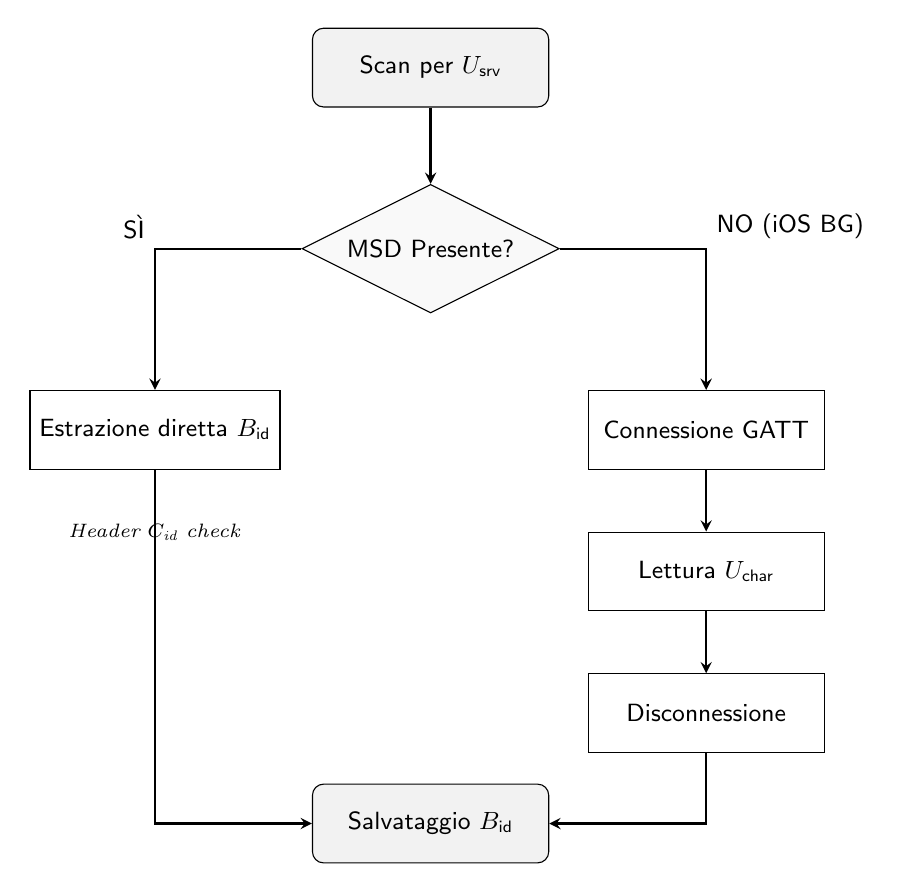
\begin{tikzpicture}[
            node distance=1.8cm,
            auto,
            font=\small\sffamily,
            % Stili dei nodi
            startstop/.style={rectangle, rounded corners, minimum width=3cm, minimum height=1cm, text centered, draw=black, fill=gray!10},
            process/.style={rectangle, minimum width=3cm, minimum height=1cm, text centered, draw=black, fill=white},
            decision/.style={diamond, aspect=2, minimum width=3cm, minimum height=1cm, text centered, draw=black, fill=gray!5},
            arrow/.style={thick,->,>=stealth}
        ]

        % Nodi
        \node (start) [startstop] {Scan per \(U_{\text{srv}}\)};
        \node (check) [decision, below of=start, yshift=-0.5cm] {MSD Presente?};

        % Ramo GAP (Sinistra)
        \node (gap_read) [process, below of=check, xshift=-3.5cm, yshift=-0.5cm] {Estrazione diretta \(B_{\text{id}}\)};
        \node (gap_note) [text width=3cm, align=center, below of=gap_read, yshift=0.5cm, font=\scriptsize\itshape] {Header \(C_{\text{id}}\) check};

        % Ramo GATT (Destra)
        \node (connect) [process, below of=check, xshift=3.5cm, yshift=-0.5cm] {Connessione GATT};
        \node (read_char) [process, below of=connect] {Lettura \(U_{\text{char}}\)};
        \node (disconnect) [process, below of=read_char] {Disconnessione};

        % Convergenza
        \node (save) [startstop, below of=check, yshift=-5.5cm] {Salvataggio \(B_{\text{id}}\)};

        % Collegamenti
        \draw [arrow] (start) -- (check);

        % Freccia SI
        \draw [arrow] (check) -| node[anchor=south east] {SÌ} (gap_read);
        \draw [arrow] (gap_read) |- (save);

        % Freccia NO
        \draw [arrow] (check) -| node[anchor=south west] {NO (iOS BG)} (connect);
        \draw [arrow] (connect) -- (read_char);
        \draw [arrow] (read_char) -- (disconnect);
        \draw [arrow] (disconnect) |- (save);

    \end{tikzpicture}
    \caption{Flusso logico di acquisizione dati}
    \label{fig:hybrid_discovery}
\end{figure}

\section{Architettura dei Moduli Software}
Il sistema è strutturato secondo il pattern \emph{Native-Controlled}. In questo modello architetturale, i moduli nativi (iOS e Android) possiedono il controllo del flusso di esecuzione e delle risorse hardware, mentre il modulo condiviso (KMM) funge da nucleo logico passivo.

Di seguito sono definiti i moduli principali e le loro responsabilità.

\subsection{Strato Condiviso (KMM)}
Il modulo \texttt{:shared} centralizza la logica di dominio, la persistenza dei dati grezzi e la gestione dello stato applicativo, garantendo la totale uniformità comportamentale tra le piattaforme.

\textbf{Definizione (\texttt{Core}):}
Sia \texttt{Core} il componente di facciata (\emph{Facade}) con solo stato volatile (cache in RAM), nessuno stato persistente che funge da unico punto di ingresso per i driver nativi.
\emph{Uso:} Gestione del protocollo di trasporto. Le sue responsabilità sono:
\begin{itemize}
    \item validare formalmente i pacchetti BLE ricevuti e applicare la logica di deduplica volatile (Cache);
    \item calcolare e fornire il payload \(B_{\text{id}}\) corrente basandosi sulla sincronizzazione temporale e sul batch locale.
\end{itemize}

\textbf{Definizione (\texttt{SecureRepository}):}
Sia \texttt{SecureRepository} il componente responsabile della persistenza sicura dei dati grezzi.
\emph{Uso:} Gestione del database locale cifrato (I/O su disco). Le sue responsabilità sono:
\begin{itemize}
    \item memorizzare il materiale crittografico per l'advertising (batch dei payload);
    \item mantenere la coda FIFO persistente dei pacchetti rilevati in attesa di invio al backend.
\end{itemize}

\textbf{Definizione (\texttt{ResolvedRepository}):}
Sia \texttt{ResolvedRepository} il componente che gestisce lo stato applicativo di alto livello.
\emph{Uso:} Sorgente di verità per l'interfaccia utente (UI). Le sue responsabilità sono:
\begin{itemize}
    \item aggregare le risposte del backend e mantenere l'insieme dinamico degli utenti risolti (\(\mathcal{A}\));
    \item applicare la logica di decadimento temporale (Time-To-Live) per rimuovere dalla vista gli utenti non più rilevati.
\end{itemize}

\subsection{Modulo Android (\texttt{:androidApp})}
Il modulo Android è progettato per garantire l'esecuzione continua in background tramite i servizi di sistema.

\textbf{Definizione (\texttt{BleService}):}
Sia \texttt{BleService} un componente architetturale di tipo \emph{Foreground Service}.
\emph{Uso:} È il componente che sopravvive alla chiusura dell'interfaccia grafica. Le sue responsabilità sono:
\begin{itemize}
    \item mantenere attivo il processo dell'applicazione;
    \item gestire le istanze dei driver \texttt{BluetoothLeAdvertiser} e \texttt{BluetoothLeScanner};
    \item coordinare le chiamate verso \texttt{Core} in base agli eventi di sistema (timer e callback BLE).
\end{itemize}

\textbf{Definizione (\texttt{GattClientManager}):}
Sia \texttt{GattClientManager} un componente ausiliario per la gestione delle connessioni.
\emph{Uso:} Gestisce le connessioni GATT puntuali. Le sue responsabilità sono:
\begin{itemize}
    \item effettuare la connessione verso dispositivi che non espongono dati in modalità GAP (es. iOS Background);
    \item leggere la caratteristica specifica ed estrarne il payload.
\end{itemize}

\subsection{Modulo iOS (\texttt{:iosApp})}
Il modulo iOS è strutturato per conformarsi al ciclo di vita rigoroso del framework CoreBluetooth.

\textbf{Definizione (\texttt{BleController}):}
Sia \texttt{BleController} il componente singleton che gestisce lo stack Bluetooth.
\emph{Uso:} Agisce da \emph{Delegate} per gli eventi di sistema. Le sue responsabilità sono:
\begin{itemize}
    \item configurare e gestire il \texttt{CBCentralManager} (scansione) e il \texttt{CBPeripheralManager} (trasmissione);
    \item implementare la logica di \emph{State Restoration} per garantire il riavvio silenzioso dell'app in background da parte del sistema operativo;
    \item orchestrare la strategia di discovery ibrida (GAP/GATT) interfacciandosi con \texttt{Core}.
\end{itemize}


\section{Strato Condiviso (KMM)}
Il modulo \texttt{:shared} è sviluppato in Kotlin puro (Kotlin/Common). Agisce come un sistema deterministico privo di dipendenze dirette dal sistema operativo: a parità di stessi input, stesso tempo logico e stesso stato persistente, produce output identici e trasformazioni di stato identiche.

\textbf{Definizione (\(B_{\text{id}}\)):}
Sia
\[
    B_{\text{id}} \in \{0,1\}^{128}
\]
l’identificativo BLE cifrato trasmesso e ricevuto via radio.
Definito in \emph{Architettura BLE lato Client e Server}.

\subsection{Core}
Il componente \texttt{Core} implementa la logica di business pura e funge da orchestratore deterministico tra (i) input dei driver nativi e (ii) stato locale persistente gestito dai repository.
Le interazioni con il backend avvengono tramite chiamate sincrone/asincrone effettuate dal client HTTP condiviso (KMM), ma \texttt{Core} resta privo di dipendenze dal ciclo di vita del sistema operativo: scheduling, timer e politiche di retry/backoff sono responsabilità del layer nativo.

\subsubsection{Modello Temporale}
Questa logica governa la selezione del payload da trasmettere basandosi sul tempo UTC.

\textbf{Definizione (\(t_{\text{unix}}\)):}
Sia
\[
    t_{\text{unix}} \in \mathbb{N}, \qquad [t_{\text{unix}}] = \si{\second},
\]
il tempo corrente in secondi trascorsi dal 1 gennaio 1970.
Definito in \emph{Architettura BLE lato Client e Server}.

\textbf{Definizione (\(\Delta t_{\text{slot}}\)):}
Sia
\[
    \Delta t_{\text{slot}} = \SI{600}{\second} = \SI{10}{\minute}
\]
la durata di uno slot temporale.
Definito in \emph{Architettura BLE lato Client e Server}.

\textbf{Definizione (\(S_{\text{slot}}\)):}
Sia
\[
    S_{\text{slot}}
    = \left\lfloor \frac{t_{\text{unix}}}{\Delta t_{\text{slot}}} \right\rfloor
    \in \mathbb{N}
\]
l'indice dello slot temporale corrente.
Definito in \emph{Architettura BLE lato Client e Server}.

\textbf{Procedura (\texttt{getCurrentBid}):}
Sia
\[
    \texttt{getCurrentBid}: \emptyset \rightarrow \{0,1\}^{128} \cup \{\texttt{null}\}
\]
la funzione invocata dai timer nativi per ottenere il payload da advertising nello slot corrente.

\textbf{Algoritmo:}
\begin{enumerate}
    \item \textbf{Calcolo Slot}:
          Si calcola \(S_{\text{slot}}\) a partire da \(t_{\text{unix}}\) e \(\Delta t_{\text{slot}}\).

    \item \textbf{Query Repository}:
          Si interroga la relazione \(\mathcal{T}_{\text{batch}}\) (definita in \emph{SecureRepository}).
          Si definisce
          \[
              R = \{\, b \mid (s,b)\in \mathcal{T}_{\text{batch}} \land s = S_{\text{slot}} \,\}.
          \]
          Per vincolo di chiave primaria su \(s\) (vedi \emph{SecureRepository}) vale \(|R| \le 1\).

    \item \textbf{Restituzione}:
          \[
              \text{Return } \begin{cases}
                  b             & \text{se } R = \{b\}     \\
                  \texttt{null} & \text{se } R = \emptyset
              \end{cases}
          \]
\end{enumerate}

\subsubsection{Memoria Volatile}
Questa logica governa l’ingestione dei pacchetti osservati, applicando un rate-limiting in RAM per proteggere l’I/O del dispositivo ed evitare accodamenti ridondanti.
Nel modello si assume che i driver nativi validino il formato e forniscano in input sempre un \(B_{\text{id}}\) in \(\{0,1\}^{128}\).

\textbf{Definizione (\(b\)):}
Sia
\[
    b \in \{0,1\}^{128}
\]
un payload ricevuto dai driver nativi, cioè un’istanza di \(B_{\text{id}}\).

\textbf{Definizione (\(\tau\)):}
Sia
\[
    \tau = \frac{\Delta t_{\text{slot}}}{6}
\]
la finestra minima tra due inserimenti dello stesso payload in coda.


\textbf{Definizione (\(\mathcal{C}\)):}
Sia
\[
    \mathcal{C} \subset \{0,1\}^{128} \times \mathbb{N}
\]
la cache volatile, che associa a ciascun payload \(b\) l’ultimo timestamp \(t\) di ingestione.

\textbf{Predicato (\(\text{hit}\)):}
\[
    \text{hit}(b) \iff \exists (b, t_{\text{ins}}) \in \mathcal{C}\ \mid\ (t_{\text{unix}} - t_{\text{ins}}) < \tau.
\]
la funzione che verifica la presenza recente di un payload, definita da:

\textbf{Procedura (\texttt{ingestPacket}):}
Sia
\[
    \texttt{ingestPacket}: \{0,1\}^{128} \rightarrow \emptyset
\]
la funzione di ingestione dei pacchetti rilevati.

\textbf{Algoritmo:}
\begin{enumerate}
    \item \textbf{Check Cache}:
          Se \(\text{hit}(b)\) è vera, termina.

    \item \textbf{Commit}:
          Il payload viene accodato in \(\mathcal{T}_{\text{queue}}\) (definita in \emph{SecureRepository}) tramite la procedura persistente \texttt{SecureRepository.enqueue}.
          La semantica è:
          \[
              \exists\, k_{\text{new}} \in \mathbb{N}
              \ \text{tale che}\
              k_{\text{new}} > k \ \ \forall (k,\widetilde{b})\in\mathcal{T}_{\text{queue}},
          \]
          e si esegue
          \[
              \mathcal{T}_{\text{queue}} \leftarrow \mathcal{T}_{\text{queue}} \cup \{ (k_{\text{new}}, b) \}.
          \]
          In implementazione, \(k_{\text{new}}\) è assegnato dal DB tramite chiave autoincrementale.

    \item \textbf{Aggiornamento Cache}:
          \[
              \mathcal{C} \leftarrow
              \Bigl(\mathcal{C} \setminus \{(b,t)\mid (b,t)\in\mathcal{C}\}\Bigr)
              \cup \{(b, t_{\text{unix}})\}.
          \]
\end{enumerate}

\subsubsection{Sincronizzazione Batch}
Questa logica governa quando e come aggiornare il batch locale usato dall’advertising, garantendo che la funzione \texttt{getCurrentBid} sia definita (non-\texttt{null}) per lo slot corrente in condizioni di connettività.

\textbf{Definizione (\(T_{\text{batch}}\)):}
Sia
\[
    T_{\text{batch}} = \SI{24}{\hour}
\]
la durata di validità di un batch di \(B_{\text{id}}\) inviato dal backend al client.
Definito in \emph{Architettura BLE lato Client e Server}.

\textbf{Definizione (\(N_{\text{batch}}\)):}
Sia
\[
    N_{\text{batch}} = \frac{T_{\text{batch}}}{\Delta t_{\text{slot}}}
\]
il numero di \(B_{\text{id}}\) contenuti in un batch.
Definito in \emph{Architettura BLE lato Client e Server}.

\textbf{Definizione (\(\mathbf{B}\)):}
Sia
\[
    \mathbf{B}
    = \bigl(B_{\text{id},j}\bigr)_{j=1}^{N_{\text{batch}}},
    \qquad B_{\text{id},j} \in \{0,1\}^{128},
\]
una sequenza ordinata di payload ricevuta dal backend.
Definito in \emph{Architettura BLE lato Client e Server}.

\textbf{Definizione (\(S_1\)):}
Sia
\[
    S_1 \in \mathbb{N}
\]
l’indice del primo slot coperto dal batch \(\mathbf{B}\).
Definito in \emph{Architettura BLE lato Client e Server}.

\textbf{Procedura (\texttt{ensureAdvertisingBatch}):}
Sia
\[
    \texttt{ensureAdvertisingBatch}: \emptyset \rightarrow \emptyset
\]
la procedura invocata periodicamente o su eventi (primo avvio, login, \texttt{getCurrentBid}=\texttt{null}) per garantire copertura del batch locale.

\textbf{Algoritmo:}
\begin{enumerate}
    \item \textbf{Calcolo Slot}:
          Si calcola \(S_{\text{slot}}\).

    \item \textbf{Controllo Copertura}:
          Si definisce
          \[
              S_{\max} =
              \max\Bigl(\{\, s \in \mathbb{N} \mid \exists b:\ (s,b)\in\mathcal{T}_{\text{batch}} \,\}\Bigr)
          \]
          se \(\mathcal{T}_{\text{batch}}\neq \emptyset\).
          La copertura è considerata \emph{insufficiente} se vale almeno una delle seguenti condizioni:
          \begin{enumerate}[label=(\alph*), nosep]
              \item \(\mathcal{T}_{\text{batch}} = \emptyset\);
              \item \(\not\exists\, b:\ (S_{\text{slot}},b)\in\mathcal{T}_{\text{batch}}\);
              \item \(\mathcal{T}_{\text{batch}}\neq \emptyset\) e \(S_{\max} - S_{\text{slot}} < \frac{N_{\text{batch}}}{6}\).
          \end{enumerate}

    \item \textbf{Fetch dal backend (solo se insufficiente)}:
          Se la copertura è insufficiente, si richiede al backend un nuovo batch \((S_1,\mathbf{B})\) tale che lo slot corrente sia coperto:
          \[
              S_1 \le S_{\text{slot}} \le S_1 + N_{\text{batch}} - 1.
          \]
          In caso di errore o assenza di connettività, lo stato locale non viene modificato.

    \item \textbf{Commit Atomico}:
          Se il fetch ha successo, si invoca \texttt{SecureRepository.replaceBatch}\((S_1,\mathbf{B})\), che sostituisce \(\mathcal{T}_{\text{batch}}\) in un’unica transazione (vedi \emph{SecureRepository}).
\end{enumerate}

\subsubsection{Sincronizzazione Coda}
Questa logica governa l’invio dei payload osservati al backend e l’aggiornamento dello stato UI in modo idempotente e consistente rispetto alla FIFO persistente, con una semantica \(1{:}1\) tra chiamata HTTP e payload processato.

\textbf{Procedura (\texttt{syncQueue}):}
Sia
\[
    \texttt{syncQueue}: \emptyset \rightarrow \emptyset
\]
la procedura invocata periodicamente dai layer nativi.

\textbf{Algoritmo:}
\begin{enumerate}
    \item \textbf{Selezione Testa FIFO}:
          Si invoca \(\texttt{SecureRepository.peekHead}()\).
          Se restituisce \texttt{null}, si invoca comunque
          \[
              \texttt{ResolvedRepository.pruneActiveSet}().
          \]
          e termina.
          Altrimenti si ottiene \((k_0,b_0)\) come testa FIFO da processare.

    \item \textbf{Chiamata Backend (singolo payload)}:
          Si invia al backend il solo payload \(b_0\) per ottenere, al più, un singolo match applicativo.

          La risposta viene modellata come un valore opzionale
          \[
              R_{\text{srv}} \in \mathcal{M} \cup \{\bot\}.
          \]
          dove \(\mathcal{M}\) è definito in \emph{ResolvedRepository} (match positivo per un utente) e \(\bot\) rappresenta “nessun match” (payload non risolvibile o privo di utente associato).

          In caso di errore di rete, timeout o risposta non valida, la procedura termina senza modificare lo stato persistente:
          \[
              \mathcal{T}_{\text{queue}} \text{ resta invariata.}
          \]

    \item \textbf{Ack e Dequeue Atomico}:
          Se la chiamata ha avuto esito tecnico positivo, si invoca in transazione
          \[
              \texttt{SecureRepository.deleteByKey}(k_0).
          \]

    \item \textbf{Aggiornamento Stato UI}:
          Se \(R_{\text{srv}} = m\), si invoca
          \[
              \texttt{ResolvedRepository.onMatchFound}(m).
          \]

          Indipendentemente dal fatto che vi sia stato match o meno, al termine si invoca
          \[
              \texttt{ResolvedRepository.pruneActiveSet}()
          \]
          per applicare il decadimento temporale e mantenere \(\mathcal{A}\) coerente rispetto a \(t_{\text{unix}}\).
\end{enumerate}


\subsection{SecureRepository}
Il repository gestisce lo stato persistente dei dati grezzi (\emph{Raw Data}) e costituisce l’unico componente autorizzato a effettuare I/O su disco.
Espone due strutture persistenti: (i) batch per l’advertising e (ii) coda FIFO di ingestione.
Ogni modifica su disco avviene in transazione ACID (SQLite), in modo che gli invarianti dichiarati siano preservati anche in caso di crash.

\subsubsection{Implementazione DB}
La persistenza è implementata tramite un database SQLite cifrato \emph{at-rest}.
\begin{itemize}
    \item Il driver DB è fornito al KMM dal layer nativo (Android/iOS).
    \item La chiave di cifratura del DB è generata e conservata in un contenitore sicuro del sistema operativo (Android Keystore / iOS Keychain) e non transita mai in log né in storage non protetti.
    \item Le tabelle sono indicizzate sulle rispettive chiavi primarie per garantire:
          \begin{itemize}[nosep]
              \item lookup \(O(1)\) sul batch (per \(s\));
              \item lettura testa FIFO tramite indice su k: ORDER BY k ASC LIMIT 1
          \end{itemize}
\end{itemize}

\subsubsection{Advertising Batch}
Struttura \emph{read-optimized} per il recupero \(O(1)\) del payload da trasmettere nello slot corrente.

\textbf{Definizione (\(s\)):}
Sia
\[
    s \in \mathbb{N}
\]
un indice di slot temporale.
Definito in \emph{Architettura BLE lato Client e Server} tramite la discretizzazione \(S_{\text{slot}}\).

\textbf{Definizione (\(\mathcal{T}_{\text{batch}}\)):}
Sia
\[
    \mathcal{T}_{\text{batch}} \subset \mathbb{N} \times \{0,1\}^{128}
\]
la relazione persistente che associa a ciascun indice di slot \(s\) il payload \(b\) da trasmettere in quello slot.

\textbf{Vincolo (chiave primaria su \(s\)):}
\[
    \forall (s,b),(s,b') \in \mathcal{T}_{\text{batch}} \;\Rightarrow\; b=b'.
\]

\textbf{Vincolo (cardinalità massima):}
\[
    |\mathcal{T}_{\text{batch}}| \le N_{\text{batch}}.
\]
\emph{Uso:} garantisce che il batch locale non cresca senza bound; in condizioni normali contiene esattamente \(N_{\text{batch}}\) righe.

\textbf{Procedura (\texttt{replaceBatch}):}
Sia
\[
    \texttt{replaceBatch}: \mathbb{N} \times \Bigl(\{0,1\}^{128}\Bigr)^{N_{\text{batch}}} \rightarrow \emptyset
\]
la procedura che sostituisce atomicamente \(\mathcal{T}_{\text{batch}}\) con un nuovo batch \((S_1,\mathbf{B})\).

\textbf{Algoritmo (transazione unica):}
\begin{enumerate}
    \item Si esegue \(\mathcal{T}_{\text{batch}} \leftarrow \emptyset\).
    \item Per ogni \(j \in \{1,\dots,N_{\text{batch}}\}\) si inserisce:
          \[
              \mathcal{T}_{\text{batch}} \leftarrow \mathcal{T}_{\text{batch}} \cup \{(S_1 + (j-1),\, B_{\text{id},j})\}.
          \]
\end{enumerate}

\subsubsection{Ingestion Queue}
Struttura \emph{write-optimized} per l’accumulo persistente dei payload osservati in attesa di invio al backend.
L’ordine FIFO è indotto dalla chiave sequenziale crescente.

\textbf{Definizione (\(k\)):}
Sia
\[
    k \in \mathbb{N}
\]
un indice sequenziale persistente, monotono crescente, utilizzato come chiave primaria della coda.

\textbf{Definizione (\(\mathcal{T}_{\text{queue}}\)):}
Sia
\[
    \mathcal{T}_{\text{queue}} \subset \mathbb{N} \times \{0,1\}^{128}
\]
la relazione persistente che modella la FIFO.

\textbf{Vincolo (chiave primaria su \(k\)):}
\[
    \forall (k,b),(k,b') \in \mathcal{T}_{\text{queue}} \;\Rightarrow\; b=b'.
\]

\textbf{Proprietà (FIFO indotta da \(k\)):}
Qualsiasi operazione di lettura/esportazione deve considerare gli elementi in ordine crescente di \(k\), a partire dal minimo \(k\) presente.

\textbf{Definizione (\(Q_{\max}\)):}
Sia
\[
    Q_{\max} = 50000
\]
la capacità massima della coda persistente.
\emph{Uso:} limite di sicurezza per prevenire crescita illimitata in condizioni offline prolungate.

\textbf{Vincolo (capacità):}
\[
    |\mathcal{T}_{\text{queue}}| \le Q_{\max}.
\]

\textbf{Procedura (\texttt{enqueue}):}
Sia
\[
    \texttt{enqueue}: \{0,1\}^{128} \rightarrow \emptyset
\]
la procedura di inserimento persistente.

\textbf{Algoritmo (transazione unica):}
\begin{enumerate}
    \item \textbf{Enforce Cap}:
          Se \(|\mathcal{T}_{\text{queue}}| = Q_{\max}\), si elimina il più vecchio elemento:
          \[
              k_{\min} = \min\{\, k \in \mathbb{N} \mid \exists b:\ (k,b)\in \mathcal{T}_{\text{queue}} \,\},
          \]
          e, per vincolo di chiave primaria su \(k\), esiste un unico \(b_{\min}\) tale che \((k_{\min},b_{\min})\in \mathcal{T}_{\text{queue}}\).
          Si esegue quindi:
          \[
              \mathcal{T}_{\text{queue}} \leftarrow \mathcal{T}_{\text{queue}} \setminus \{(k_{\min},b_{\min})\}.
          \]

    \item \textbf{Insert}:
          Si inserisce un nuovo elemento con chiave crescente assegnata dal DB:
          \[
              \exists\, k_{\text{new}}\in\mathbb{N} \text{ con } k_{\text{new}} > k\ \forall (k,\widetilde{b})\in\mathcal{T}_{\text{queue}},
          \]
          \[
              \mathcal{T}_{\text{queue}} \leftarrow \mathcal{T}_{\text{queue}} \cup \{(k_{\text{new}}, b)\}.
          \]
\end{enumerate}

\textbf{Procedura (\texttt{peekHead}):}
Sia
\[
    \texttt{peekHead}: \emptyset \rightarrow (\mathbb{N} \times \{0,1\}^{128}) \cup \{\texttt{null}\}
\]
la procedura che restituisce la testa FIFO senza modificarla.
\emph{Uso:} query indicizzata \texttt{ORDER BY k ASC LIMIT 1}.

\textbf{Procedura (\texttt{deleteByKey}):}
Sia
\[
    \texttt{deleteByKey}: \mathbb{N} \rightarrow \emptyset
\]
la procedura che elimina esattamente l’elemento con chiave primaria \(k\), in transazione.
\emph{Uso:} \texttt{DELETE FROM queue WHERE k = :k}.


\subsection{ResolvedRepository}
Il repository gestisce lo stato applicativo di alto livello mostrato in UI: l’insieme degli utenti risolti dal backend e la loro validità temporale.
Non mantiene alcun mapping persistente \(B_{\text{id}} \rightarrow\) utente, in accordo con \emph{Architettura BLE lato Client e Server}.
Lo stato \(\mathcal{A}\) è mantenuto in memoria (volatile) e viene ricostruito esclusivamente a partire dalle risposte del backend.

\subsubsection{Modello Dati Utente}

\textbf{Definizione (\(U_{\text{view}}\)):}
Sia
\[
    U_{\text{view}} = (id_u, N_u, t_{\text{last}})
\]
una tripla che rappresenta un utente in vista UI, dove \(id_u \in \mathbb{N}\) è l’identificativo univoco restituito dal backend,
\(N_u\) è il nome visualizzato, e
\[
    t_{\text{last}} \in \mathbb{N}, \qquad [t_{\text{last}}]=\si{\second},
\]
è il timestamp Unix dell’ultimo aggiornamento valido.

\textbf{Definizione (\(\mathbb{S}\)):}
Sia \[\mathbb{S}\] l’insieme delle stringhe UTF-8 con lunghezza massima \(64\) caratteri.

\textbf{Definizione (\(\mathcal{A}\)):}
Sia
\[
    \mathcal{A} \subset \mathbb{N} \times \mathbb{S} \times \mathbb{N}
\]
l’insieme dinamico degli utenti attualmente considerati vicini.


\textbf{Vincolo (unicità per \(id_u\)):}
\[
    \forall (id_u,N,t),(id_u,N',t') \in \mathcal{A} \;\Rightarrow\; (N,t)=(N',t').
\]

\subsubsection{Logica di Aggiornamento}

\textbf{Definizione (\(\mathcal{M}\)):}
Sia
\[
    \mathcal{M} = \mathbb{N} \times \mathbb{S}
\]
l’insieme dei match possibili restituiti dal backend.

\textbf{Definizione (\(m\)):}
Sia
\[
    m=(id_u, N_u)\in\mathcal{M}
\]
un match (istanza) restituito dal backend.

\textbf{Procedura (\texttt{onMatchFound}):}
Sia
\[
    \texttt{onMatchFound}: \mathcal{M} \rightarrow \emptyset
\]
la procedura invocata al tempo corrente \(t_{\text{unix}}\).

\textbf{Algoritmo:}
\begin{enumerate}
    \item Si cerca \(U_{\text{view}} \in \mathcal{A}\) tale che \(U_{\text{view}}.id_u = m.id_u\).

    \item \textbf{Se esiste} \(U_{\text{view}}=(id_u,\widetilde{N},\widetilde{t})\):
          si aggiorna \(\mathcal{A}\) sostituendo tale elemento con
          \[
              (id_u, m.N_u, \max(\widetilde{t}, t_{\text{unix}})).
          \]

    \item \textbf{Se non esiste}:
          si inserisce in \(\mathcal{A}\) l’elemento
          \[
              (M.id_u, m.N_u, t_{\text{unix}}).
          \]

    \item Se \(\mathcal{A}\) è cambiato, si notifica la UI.
\end{enumerate}

\subsubsection{Logica di Pruning}

\textbf{Definizione (\(\tau_{\text{vis}}\)):}
Sia
\[
    \tau_{\text{vis}} = \frac{\Delta t_{\text{slot}}}{3}
\]
il tempo massimo di permanenza senza refresh.
\emph{Uso:} scelta tale che \(\tau < \tau_{\text{vis}}\), evitando che la deduplica di ingestione riduca la reattività della vista.

\textbf{Procedura (\texttt{pruneActiveSet}):}
Sia
\[
    \texttt{pruneActiveSet}: \emptyset \rightarrow \emptyset
\]
la procedura invocata periodicamente al tempo corrente \(t_{\text{unix}}\).

\textbf{Algoritmo:}
\begin{enumerate}
    \item Si identifica il sottoinsieme scaduto:
          \[
              \mathcal{A}_{\text{exp}}
              =
              \{\, (id_u,N_u,t_{\text{last}})\in\mathcal{A}
              \mid (t_{\text{unix}} - t_{\text{last}}) \ge \tau_{\text{vis}} \,\}.
          \]

    \item Si rimuove il sottoinsieme scaduto:
          \[
              \mathcal{A} \leftarrow \mathcal{A} \setminus \mathcal{A}_{\text{exp}}.
          \]

    \item Se \(\mathcal{A}_{\text{exp}} \neq \emptyset\), si notifica la UI.
\end{enumerate}

\section{Modulo iOS (\texttt{:iosApp})}
Il modulo iOS implementa la logica BLE nativa tramite \emph{CoreBluetooth}, rispettando i vincoli di esecuzione in background e la peculiarità iOS per cui il campo \emph{Manufacturer Specific Data} (MSD) non è affidabile in background. Il controllo del flusso resta nativo: il modulo invoca unicamente le procedure pubbliche del modulo condiviso (\texttt{Core}) e preserva la semantica FIFO persistente della coda \(\mathcal{T}_{\text{queue}}\) e del batch \(\mathcal{T}_{\text{batch}}\) (definiti nello \emph{Strato Condiviso (KMM)}).

\subsection{\texttt{BleController}}
\texttt{BleController} è un singleton che possiede e coordina:
\begin{itemize}[nosep]
    \item un \texttt{CBCentralManager} per scanning e connessioni GATT (ruolo \emph{central});
    \item un \texttt{CBPeripheralManager} per advertising e server GATT (ruolo \emph{peripheral});
    \item lo scheduling delle invocazioni periodiche/event-driven verso KMM:
          \\ \texttt{Core.ensureAdvertisingBatch}, \texttt{Core.getCurrentBid}, \texttt{Core.ingestPacket}, \\ \texttt{Core.syncQueue}.
\end{itemize}
Tutte le invocazioni verso KMM e tutte le transizioni operative BLE sono serializzate su un’unica coda di esecuzione (single-queue), così che, a parità di stessi eventi nativi e stesso stato persistente, gli effetti osservabili siano deterministici.

\subsubsection{Stato foreground/background e commutazione deterministica}
La commutazione FG/BG è guidata dallo stato dell’app iOS esposto dal lifecycle (\texttt{UIApplication}/\texttt{UIScene}).
\texttt{BleController} non deduce FG/BG dallo stack BLE: aggiorna uno stato interno consultando e ricevendo i callback del sistema operativo.

\textbf{Definizione (\(\sigma\)):}
Sia
\[
    \sigma \in \{\mathrm{FG}, \mathrm{BG}\}
\]
lo stato corrente dell’applicazione iOS.
\emph{Uso:} determina la modalità di advertising locale e stabilisce se il payload applicativo debba transitare in MSD (\(\mathrm{FG}\)) oppure via GATT (\(\mathrm{BG}\)).

\paragraph{Regola (mappatura lifecycle \(\to \sigma\)):}
\(\sigma=\mathrm{FG}\) se e solo se l’app è in stato \emph{foreground attivo} (es. \texttt{applicationState == active} oppure \texttt{scene.activationState == foregroundActive}). In tutti gli altri casi (\texttt{inactive} inclusa), si impone \(\sigma=\mathrm{BG}\) per sicurezza operativa (evita di assumere MSD affidabile durante transizioni, lock screen o interruzioni).

\paragraph{Trigger (transizioni):}
\texttt{BleController} aggiorna \(\sigma\) e applica la riconfigurazione al verificarsi di:
\begin{itemize}[nosep]
    \item ingresso in background (\texttt{didEnterBackground}/\texttt{sceneDidEnterBackground});
    \item rientro in foreground (\texttt{willEnterForeground}/\texttt{sceneWillEnterForeground} \\ e successivo \texttt{didBecomeActive}/\texttt{sceneDidBecomeActive});
    \item transizione a stato non attivo (\texttt{willResignActive}/\texttt{sceneWillResignActive}), che viene trattata come \(\mathrm{BG}\).
\end{itemize}

\subsubsection{Implementazione della matrice BLE}
La matrice di comportamento è implementata come scelta deterministica tra \(\text{GAP}\) e \(\text{GATT}\) in base a \(\sigma\) (per trasmissione) e alla presenza dell’MSD (per ricezione). Le costanti \(U_{\text{srv}}, U_{\text{char}}, C_{\text{id}}\) sono definite nella sezione \emph{Matrice di comportamento BLE} di questo documento.

\textbf{Definizione (\(\text{msdPresent}\)):}
Sia
\[
    \text{msdPresent} \in \{\text{Vero}, \text{Falso}\}
\]
il predicato che vale \text{Vero} se e solo se il report di discovery contiene un blocco MSD tale che (i) i primi \SI{2}{\byte} sono \(\texttt{B1 00}\) (little-endian di \(C_{\text{id}}=\texttt{0x00B1}\)) e (ii) la lunghezza totale del dato applicativo è \(\SI{18}{\byte}\) (header \(C_{\text{id}}\) + \(\SI{16}{\byte}\)).
\emph{Uso:} seleziona la lettura diretta (GAP) oppure il fallback connesso (GATT) in scanning.

\paragraph{Regola (Advertising iOS):}
\begin{itemize}[nosep]
    \item se \(\sigma=\mathrm{FG}\), l’advertising è \(\text{GAP}\): in advertisement sono presenti \(U_{\text{srv}}\) e l’MSD che porta \(B_{\text{id}}\);
    \item se \(\sigma=\mathrm{BG}\), l’advertising è \(\text{GATT}\): in advertisement è presente \(U_{\text{srv}}\) (discovery e filtro), mentre \(B_{\text{id}}\) è leggibile via caratteristica \(U_{\text{char}}\) del servizio pubblicato.
\end{itemize}

\paragraph{Regola (Scanning iOS):}
lo scanning è sempre filtrato su \(U_{\text{srv}}\). Per ogni peripheral scoperto:
\begin{itemize}[nosep]
    \item se \(\text{msdPresent}=\text{Vero}\), si estrae \(B_{\text{id}}\) in \(\text{GAP}\) e si invoca \texttt{Core.ingestPacket};
    \item se \(\text{msdPresent}=\text{Falso}\), si attiva il fallback \(\text{GATT}\) e si legge \(U_{\text{char}}\).
\end{itemize}
Questa regola realizza la matrice in modo completo: in particolare copre il caso “trasmittente iOS in BG” dove l’MSD è assente/non affidabile, quindi \(\text{msdPresent}=\text{Falso}\Rightarrow\text{GATT}\).

\subsubsection{Precondizioni di piattaforma}
L’operatività è subordinata allo stato CoreBluetooth e ai permessi.
\begin{itemize}[nosep]
    \item Se lo stato Bluetooth non è utilizzabile (\texttt{poweredOff}/\texttt{unauthorized}/\texttt{unsupported}/\texttt{resetting}), \texttt{BleController} forza \texttt{stopAdvertising}, interrompe le sessioni GATT in corso e sospende lo scanning.
    \item Le modalità in background richiedono i \emph{Background Modes} per Bluetooth (\texttt{bluetooth-central} e \texttt{bluetooth-peripheral}) e le \emph{usage description} previste dal sistema; in assenza, gli invarianti di scheduling restano validi ma l’esecuzione in background non è garantita.
\end{itemize}
Queste condizioni non modificano mai \(\mathcal{T}_{\text{batch}}\) o \(\mathcal{T}_{\text{queue}}\) direttamente: ogni modifica persistente avviene solo tramite KMM.

\subsubsection{Inizializzazione e \emph{State Restoration}}
\texttt{BleController} inizializza \texttt{CBCentralManager} e \texttt{CBPeripheralManager} con \emph{restoration identifiers} distinti e abilita la \emph{state restoration}. Su ripristino, ricostruisce le invarianti operative in modo idempotente:
\begin{itemize}[nosep]
    \item riattiva lo scanning filtrato su \(U_{\text{srv}}\) se lo stato Bluetooth è utilizzabile;
    \item ricostruisce (se necessario) il server GATT (servizio \(U_{\text{srv}}\) + caratteristica \(U_{\text{char}}\));
    \item riallinea l’advertising alla regola imposta da \(\sigma\) (sezione successiva);
    \item riattiva i timer (sezione \emph{Scheduling}).
\end{itemize}
La \emph{restoration} non implica alcun enqueue/dequeue: la FIFO \(\mathcal{T}_{\text{queue}}\) e il batch \(\mathcal{T}_{\text{batch}}\) sono già persistenti e restano la sorgente di verità per KMM.

\subsubsection{Advertising e reconfigurazione FG/BG}
\texttt{BleController} non costruisce \(B_{\text{id}}\): richiede al KMM il payload di slot corrente tramite \texttt{Core.getCurrentBid} (definita nello \emph{Strato Condiviso (KMM)}). Il processo di advertising è deterministico e dipende da \(\sigma\).

\paragraph{Composizione MSD (solo \(\sigma=\mathrm{FG}\)):}
L’MSD trasporta un vettore di \(\SI{18}{\byte}\) definito come
\[
    D = C_{\text{id}} \ \| \ B_{\text{id}},
\]
dove \(C_{\text{id}}\) occupa i primi \(\SI{2}{\byte}\) e \(B_{\text{id}}\in\{0,1\}^{128}\) i successivi \(\SI{16}{\byte}\). In scanning la validazione è: \(|D|=\SI{18}{\byte}\) e \(D[0..1]=C_{\text{id}}\) (endianness conforme all’API nativa).

\paragraph{Procedura (applyAdvertisingMode):}
La procedura viene invocata quando:
\begin{itemize}[nosep]
    \item lo stato Bluetooth diventa utilizzabile (\texttt{poweredOn});
    \item \(\sigma\) cambia (FG\(\leftrightarrow\)BG);
    \item cambia lo slot temporale \(S_{\text{slot}}\) (sezione successiva).
\end{itemize}
I passi sono:
\begin{enumerate}
    \item invocare \texttt{Core.ensureAdvertisingBatch()} (opportunistico: se la copertura è sufficiente non produce modifiche persistenti; definita nello \emph{Strato Condiviso (KMM)});
    \item invocare \texttt{Core.getCurrentBid()}. Se restituisce \texttt{null}, eseguire \texttt{stopAdvertising} e non esporre dato applicativo (né in MSD né via \(U_{\text{char}}\)) finché un batch valido non viene ripristinato;
    \item se \texttt{Core.getCurrentBid()} restituisce un valore, allora:
          \begin{itemize}[nosep]
              \item se \(\sigma=\mathrm{FG}\): pubblicare l’advertising in \(\text{GAP}\) includendo \(U_{\text{srv}}\) e MSD \(D\);
              \item se \(\sigma=\mathrm{BG}\): pubblicare l’advertising in \(\text{GATT}\) includendo \(U_{\text{srv}}\) e assicurare l’esposizione del server GATT con caratteristica \(U_{\text{char}}\) leggibile.
          \end{itemize}
\end{enumerate}
Ogni cambio modalità forza una riconfigurazione esplicita (\texttt{stopAdvertising} seguito da \texttt{startAdvertising}) così che l’advertisement attivo sia sempre coerente con \(\sigma\).

\subsubsection{Timer di slot}
Per garantire che l’advertising in \(\mathrm{FG}\) contenga sempre il \(B_{\text{id}}\) dello slot corrente, \texttt{BleController} riallinea al cambio di slot \(S_{\text{slot}}\) (definito nello \emph{Strato Condiviso (KMM)} e in \emph{Architettura BLE lato Client e Server}).

\paragraph{Scheduling:}
Dato il tempo corrente \(t_{\text{unix}}\) e \(\Delta t_{\text{slot}}\) (definiti nello \emph{Strato Condiviso (KMM)}), \texttt{BleController} calcola localmente l’istante del prossimo bordo di slot e programma un timer a singola scadenza. Alla scadenza:
\begin{itemize}[nosep]
    \item invoca \texttt{applyAdvertisingMode} (che a sua volta richiama \texttt{Core.getCurrentBid});
    \item riprogramma il timer sul bordo successivo.
\end{itemize}
Questo elimina drift di scheduling: l’aggiornamento è sempre ancorato ai bordi di slot, non a un periodo accumulativo.

\subsubsection{Server GATT}
Quando \(\sigma=\mathrm{BG}\), il payload applicativo è esposto via GATT utilizzando \(U_{\text{srv}}\) e \(U_{\text{char}}\) (definiti nella sezione \emph{Matrice di comportamento BLE}).

\paragraph{Pubblicazione:}
\texttt{BleController} assicura che:
\begin{itemize}[nosep]
    \item esista un servizio pubblicato con UUID \(U_{\text{srv}}\);
    \item esista una caratteristica leggibile con UUID \(U_{\text{char}}\).
\end{itemize}

\paragraph{Semantica lettura caratteristica:}
Alla richiesta di lettura su \(U_{\text{char}}\), \texttt{BleController} invoca \texttt{Core.getCurrentBid()}:
\begin{itemize}[nosep]
    \item se il risultato è definito, risponde con i \(\SI{16}{\byte}\) del \(B_{\text{id}}\) corrente;
    \item se il risultato è \texttt{null}, risponde con errore GATT (dato non disponibile) e mantiene l’advertising sospeso finché \texttt{Core.ensureAdvertisingBatch()} non ripristina copertura e \texttt{Core.getCurrentBid()} torna definita.
\end{itemize}
In \(\sigma=\mathrm{BG}\) non è necessario riavviare l’advertising a ogni slot ai fini della correttezza del dato remoto: il valore letto è determinato al momento della read dalla \texttt{getCurrentBid}. Il timer di slot resta comunque attivo per gestire la riconfigurazione globale e i casi \(\sigma=\mathrm{FG}\).

\subsubsection{Scanning, acquisizione GAP e ingestione KMM}
Lo scanning è sempre filtrato su \(U_{\text{srv}}\). Per ogni evento di discovery, \texttt{BleController} applica:
\begin{enumerate}
    \item se \(\text{msdPresent}=\text{Vero}\), estrae
          \[
              B_{\text{id}} = D[2..17] \in \{0,1\}^{128}
          \]
          e invoca immediatamente \(\texttt{Core.ingestPacket}(B_{\text{id}})\);
    \item se \(\text{msdPresent}=\text{Falso}\), attiva il fallback GATT (sezione successiva).
\end{enumerate}
La deduplica e l’eventuale enqueue persistente sono interamente responsabilità di KMM tramite \texttt{Core.ingestPacket} (che applica la cache volatile e delega l’I/O a \texttt{SecureRepository.enqueue}).

\subsubsection{Fallback GATT e controllo dei tentativi}
Quando \(\text{msdPresent}=\text{Falso}\), \texttt{BleController} tenta la lettura connessa di \(U_{\text{char}}\). Per evitare tempeste di connessione e connessioni duplicate concorrenti verso lo stesso peripheral, \texttt{BleController} mantiene un throttle volatile per identificatore di peripheral (implementativamente: chiave opaca fornita da CoreBluetooth e stabile nel ciclo di vita del processo).

\textbf{Definizione (\(\mathcal{P}\)):}
Sia
\[
    \mathcal{P} \subset \{\,(\iota,t)\mid t\in\mathbb{N}\,\}
\]
una cache volatile che associa a ciascun peripheral \(\iota\) l’ultimo timestamp \(t\) di avvio di un tentativo GATT.
\emph{Uso:} limita la frequenza di tentativi GATT per peripheral con finestra minima \(\tau\) (definita nello \emph{Strato Condiviso (KMM)}), impedendo connessioni ripetute non produttive.

\paragraph{Regola (throttle):}
Un tentativo GATT verso \(\iota\) è ammesso se e solo se
\[
    \neg \exists(\iota,t)\in\mathcal{P}\ \mid\ (t_{\text{unix}}-t)<\tau.
\]
All’avvio del tentativo si aggiorna \(\mathcal{P}\) sostituendo la coppia per \(\iota\) con \((\iota,t_{\text{unix}})\).

\paragraph{Procedura (GATT read):}
Per un peripheral \(\iota\) ammesso:
\begin{enumerate}
    \item \texttt{connect} (connessione GATT);
    \item discovery del servizio \(U_{\text{srv}}\);
    \item discovery della caratteristica \(U_{\text{char}}\);
    \item \texttt{readValue} su \(U_{\text{char}}\);
    \item se la lettura restituisce un valore di \(\SI{16}{\byte}\), interpretato come \(B_{\text{id}}\in\{0,1\}^{128}\), invocare \(\texttt{Core.ingestPacket}(B_{\text{id}})\);
    \item \texttt{cancelPeripheralConnection} e cleanup della sessione.
\end{enumerate}

\paragraph{Gestione errori:}
Qualunque errore tecnico (connessione, discovery, read) termina la procedura senza invocare \texttt{Core.ingestPacket}. Il peripheral resta soggetto al throttle di \(\mathcal{P}\). I timeout sono implementati come cancellation esplicita della connessione se la sequenza non completa entro una finestra finita coerente con la logica di throttle (tipicamente non superiore alla finestra minima tra tentativi).

\subsubsection{Scheduling invocazioni KMM e garanzie}
Oltre al timer di bordo slot, \texttt{BleController} programma un timer periodico \emph{best-effort} (eseguito quando il processo ha tempo di esecuzione) con periodo \(\tau\) (definito nello \emph{Strato Condiviso (KMM)}). A ogni tick invoca in ordine:
\begin{enumerate}
    \item \texttt{Core.ensureAdvertisingBatch()};
    \item \texttt{Core.syncQueue()}.
\end{enumerate}
Non è richiesto chiamare \texttt{ResolvedRepository.pruneActiveSet} dal layer iOS: la potatura è già garantita (i) internamente a \texttt{Core.syncQueue} (definizione nello \emph{Strato Condiviso (KMM)}) quando la risoluzione viene eseguita e (ii) dalla UI/driver nativi tramite tick periodici se si desidera pruning anche in assenza totale di rete; in tal caso l’invocazione è lecita perché agisce unicamente su \(\mathcal{A}\) (volatile).

\paragraph{Garanzie:}
\begin{itemize}[nosep]
    \item \texttt{Core.ensureAdvertisingBatch} è idempotente: in assenza di rete o su errore non modifica \(\mathcal{T}_{\text{batch}}\).
    \item \texttt{Core.syncQueue} rispetta la semantica \(1{:}1\): ogni tick può processare al più un elemento (la testa FIFO) e, su errore di rete/risposta non valida, \(\mathcal{T}_{\text{queue}}\) resta invariata.
    \item \texttt{Core.ingestPacket} è l’unica via per inserire in FIFO: garantisce deduplica volatile e persistenza transazionale tramite \texttt{SecureRepository.enqueue}.
\end{itemize}

\subsubsection{Trigger evento-driven}
Oltre ai timer, \texttt{BleController} invoca KMM in punti deterministici:
\begin{itemize}[nosep]
    \item su \texttt{poweredOn}: invoca \texttt{applyAdvertisingMode} e avvia/scandisce su \(U_{\text{srv}}\);
    \item su cambio \(\sigma\) (FG\(\leftrightarrow\)BG): invoca \texttt{applyAdvertisingMode} (commuta GAP\(\leftrightarrow\)GATT) senza alterare l’invariante di scanning filtrato;
    \item su acquisizione di un payload (GAP o GATT): invoca immediatamente \texttt{Core.ingestPacket};
    \item su ripristino stato (state restoration): riapplica \texttt{applyAdvertisingMode}, riattiva scan e timers, senza eseguire side-effect persistenti diretto (solo via KMM).
\end{itemize}
La combinazione di: (i) reconfigurazione evento-driven per \(\sigma\) e per disponibilità BLE, (ii) timer di bordo slot, (iii) tick periodico \(\tau\) per batch e coda, è sufficiente a garantire che (a) l’advertising sia sempre coerente con \(\sigma\) e con lo slot corrente, (b) ogni \(B_{\text{id}}\) acquisito sia consegnato a KMM in modo idempotente, (c) la risoluzione verso backend avanzi in FIFO preservando la semantica \(1{:}1\).

\subsection{Flussi di Esecuzione}
Di seguito sono riportati i diagrammi di flusso che illustrano le principali logiche decisionali e operative del modulo iOS, in conformità con le definizioni testuali precedenti.

\subsubsection{Ciclo di Vita e Gestione Stato}
Questo diagramma mostra come \texttt{BleController} gestisce l'inizializzazione, la \emph{State Restoration} e le transizioni di stato dell'applicazione (Foreground/Background), aggiornando di conseguenza la modalità operativa \(\sigma\).

\begin{figure}[H]
    \centering
    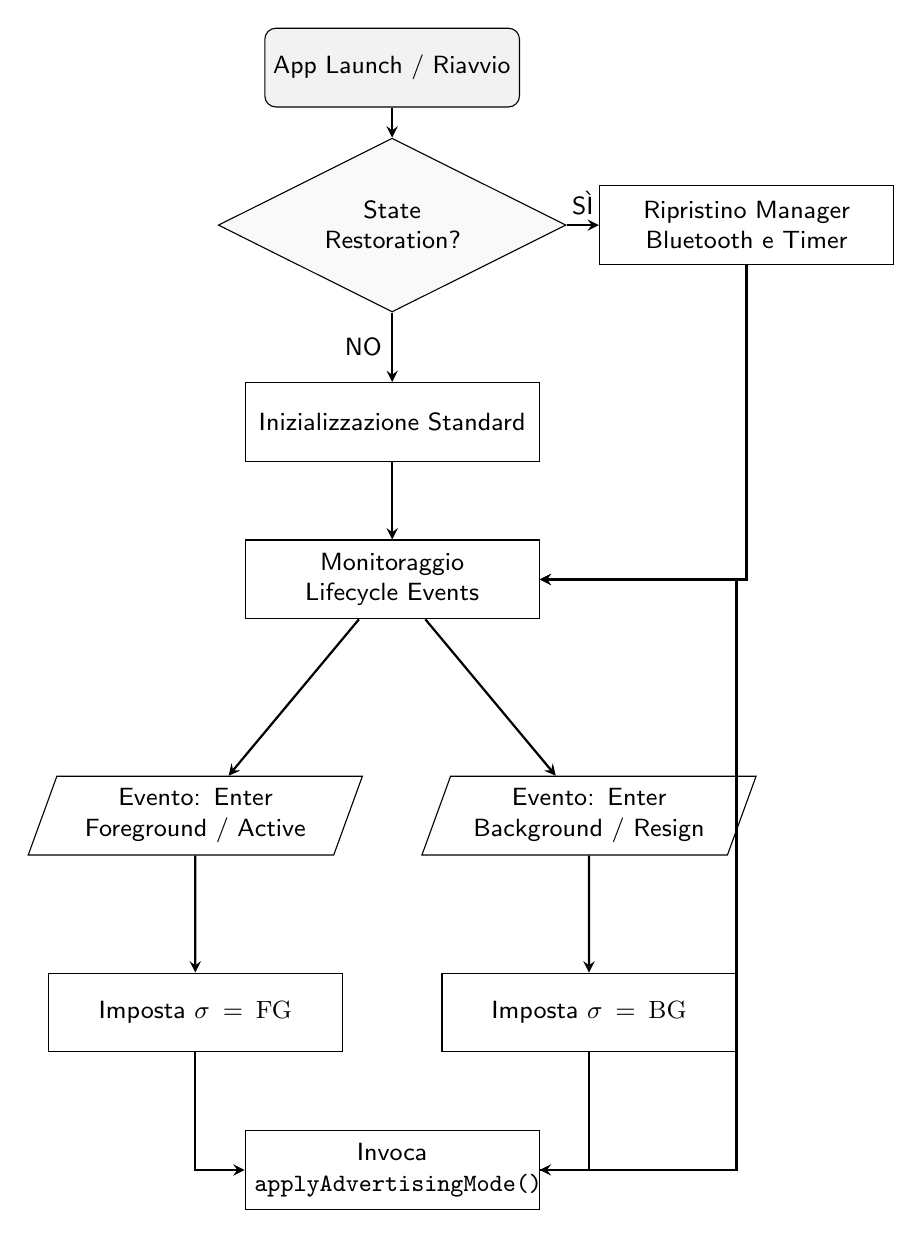
\begin{tikzpicture}[
            node distance=2cm,
            auto,
            font=\small\sffamily,
            % Definisco larghezza fissa per forzare a capo
            startstop/.style={rectangle, rounded corners, minimum width=3cm, minimum height=1cm, text centered, draw=black, fill=gray!10, text width=3cm},
            process/.style={rectangle, minimum width=3.5cm, minimum height=1cm, text centered, draw=black, fill=white, text width=3.5cm},
            decision/.style={diamond, aspect=2, minimum width=3cm, minimum height=1cm, text centered, draw=black, fill=gray!5, text width=2.5cm},
            arrow/.style={thick,->,>=stealth},
            io/.style={trapezium, trapezium left angle=70, trapezium right angle=110, minimum width=3.5cm, minimum height=1cm, text centered, draw=black, fill=white, text width=3cm}
        ]

        % Nodi
        \node (start) [startstop] {App Launch / Riavvio};
        \node (restore_check) [decision, below of=start] {State Restoration?};

        % Spostato a destra ma non troppo
        \node (restore_proc) [process, right of=restore_check, xshift=2.5cm] {Ripristino Manager Bluetooth e Timer};

        \node (init_proc) [process, below of=restore_check, yshift=-0.5cm] {Inizializzazione Standard};
        \node (lifecycle_mon) [process, below of=init_proc] {Monitoraggio Lifecycle Events};

        % Eventi affiancati ma più stretti
        \node (event_fg) [io, below of=lifecycle_mon, xshift=-2.5cm, yshift=-1cm] {Evento: Enter Foreground / Active};
        \node (event_bg) [io, below of=lifecycle_mon, xshift=2.5cm, yshift=-1cm] {Evento: Enter Background / Resign};

        \node (set_fg) [process, below of=event_fg, yshift=-0.5cm] {Imposta \(\sigma = \mathrm{FG}\)};
        \node (set_bg) [process, below of=event_bg, yshift=-0.5cm] {Imposta \(\sigma = \mathrm{BG}\)};

        % Nodo centrale in basso
        \node (apply_mode) [process, below of=lifecycle_mon, yshift=-5.5cm] {Invoca \texttt{applyAdvertisingMode()}};

        % Collegamenti
        \draw [arrow] (start) -- (restore_check);
        \draw [arrow] (restore_check) -- node[anchor=south] {SÌ} (restore_proc);
        \draw [arrow] (restore_check) -- node[anchor=east] {NO} (init_proc);

        % Collegamenti che tornano al flusso centrale
        \draw [arrow] (restore_proc) |- (lifecycle_mon);
        \draw [arrow] (init_proc) -- (lifecycle_mon);

        \draw [arrow] (lifecycle_mon) -- (event_fg);
        \draw [arrow] (lifecycle_mon) -- (event_bg);

        \draw [arrow] (event_fg) -- (set_fg);
        \draw [arrow] (event_bg) -- (set_bg);

        \draw [arrow] (set_fg) |- (apply_mode);
        \draw [arrow] (set_bg) |- (apply_mode);

        % Loop di ritorno al monitoraggio (largo a destra)
        \draw [arrow] (apply_mode.east) -- ++(2.5cm,0) |- (lifecycle_mon.east);

    \end{tikzpicture}
    \caption{Flusso del Ciclo di Vita e aggiornamento di \(\sigma\)}
    \label{fig:ios_lifecycle_flow}
\end{figure}

\newpage

\subsubsection{Logica di Advertising}
Questo diagramma dettaglia la procedura \texttt{applyAdvertisingMode}, invocata su cambi di stato, timer di slot o eventi Bluetooth. Mostra la decisione deterministica tra advertising GAP e GATT basata su \(\sigma\) e la dipendenza dal KMM.

\begin{figure}[H]
    \centering
    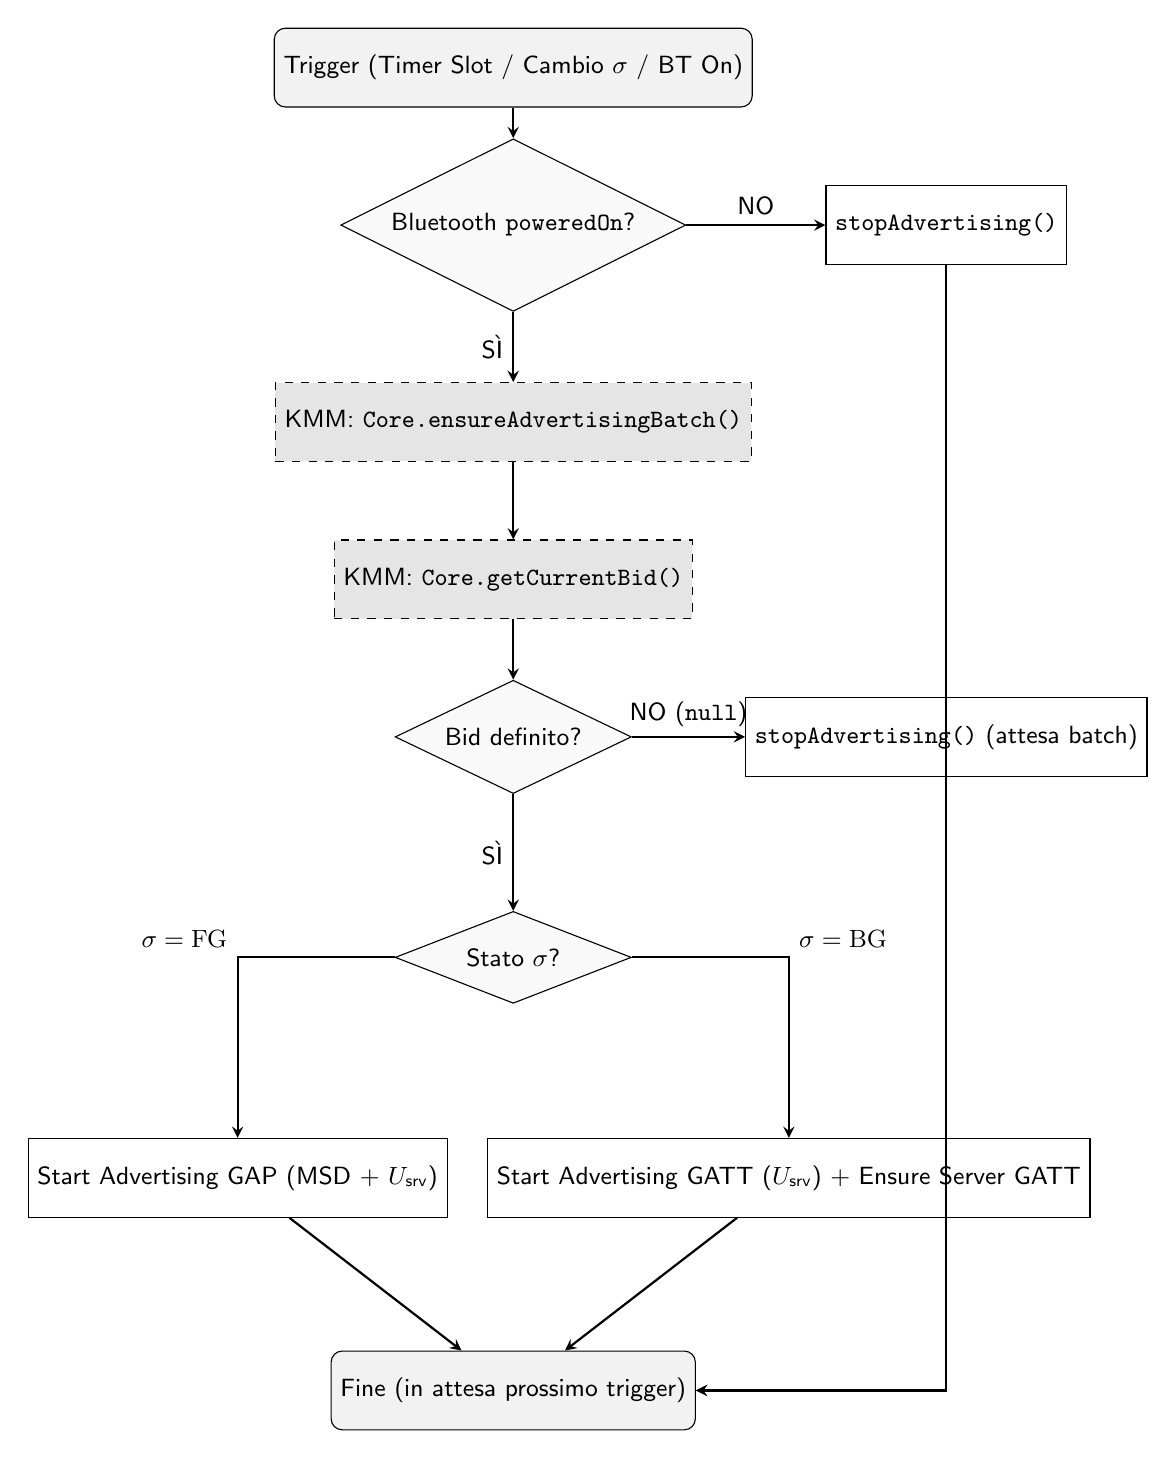
\begin{tikzpicture}[
            node distance=2cm,
            auto,
            font=\small\sffamily,
            startstop/.style={rectangle, rounded corners, minimum width=3cm, minimum height=1cm, text centered, draw=black, fill=gray!10},
            process/.style={rectangle, minimum width=3cm, minimum height=1cm, text centered, draw=black, fill=white},
            decision/.style={diamond, aspect=2, minimum width=3cm, minimum height=1cm, text centered, draw=black, fill=gray!5},
            kmm/.style={rectangle, minimum width=3cm, minimum height=1cm, text centered, draw=black, fill=gray!20, dashed},
            arrow/.style={thick,->,>=stealth}
        ]

        % Nodi
        \node (start) [startstop] {Trigger (Timer Slot / Cambio \(\sigma\) / BT On)};
        \node (bt_check) [decision, below of=start] {Bluetooth \texttt{poweredOn}?};
        \node (stop_ad_bt) [process, right of=bt_check, xshift=3.5cm] {\texttt{stopAdvertising()}};

        \node (ensure_batch) [kmm, below of=bt_check, yshift=-0.5cm] {KMM: \texttt{Core.ensureAdvertisingBatch()}};
        \node (get_bid) [kmm, below of=ensure_batch] {KMM: \texttt{Core.getCurrentBid()}};
        \node (bid_check) [decision, below of=get_bid] {Bid definito?};

        \node (stop_ad_bid) [process, right of=bid_check, xshift=3.5cm] {\texttt{stopAdvertising()} (attesa batch)};

        \node (sigma_check) [decision, below of=bid_check, yshift=-0.8cm] {Stato \(\sigma\)?};

        \node (gap_ad) [process, below of=sigma_check, xshift=-3.5cm, yshift=-0.8cm] {Start Advertising GAP (MSD + \(U_{\text{srv}}\))};
        \node (gatt_ad) [process, below of=sigma_check, xshift=3.5cm, yshift=-0.8cm] {Start Advertising GATT (\(U_{\text{srv}}\)) + Ensure Server GATT};

        \node (end) [startstop, below of=sigma_check, yshift=-3.5cm] {Fine (in attesa prossimo trigger)};

        % Collegamenti
        \draw [arrow] (start) -- (bt_check);
        \draw [arrow] (bt_check) -- node[anchor=south] {NO} (stop_ad_bt);
        \draw [arrow] (bt_check) -- node[anchor=east] {SÌ} (ensure_batch);
        \draw [arrow] (stop_ad_bt) |- (end);

        \draw [arrow] (ensure_batch) -- (get_bid);
        \draw [arrow] (get_bid) -- (bid_check);

        \draw [arrow] (bid_check) -- node[anchor=south] {NO (\texttt{null})} (stop_ad_bid);
        \draw [arrow] (stop_ad_bid) |- (end);

        \draw [arrow] (bid_check) -- node[anchor=east] {SÌ} (sigma_check);

        \draw [arrow] (sigma_check) -| node[anchor=south east] {\(\sigma=\mathrm{FG}\)} (gap_ad);
        \draw [arrow] (sigma_check) -| node[anchor=south west] {\(\sigma=\mathrm{BG}\)} (gatt_ad);

        \draw [arrow] (gap_ad) -- (end);
        \draw [arrow] (gatt_ad) -- (end);

    \end{tikzpicture}
    \caption{Flusso decisionale dell'Advertising iOS}
    \label{fig:ios_advertising_flow}
\end{figure}

\newpage

\subsubsection{Scanning, Fallback GATT e Ingestione}
Questo diagramma illustra la logica ibrida di ricezione. Mostra la gestione dell'evento di discovery, il controllo della presenza MSD, l'eventuale fallback con connessione GATT (soggetto a throttle \(\mathcal{P}\)) e l'ingestione finale del payload verso il KMM.

\begin{figure}[H]
    \centering
    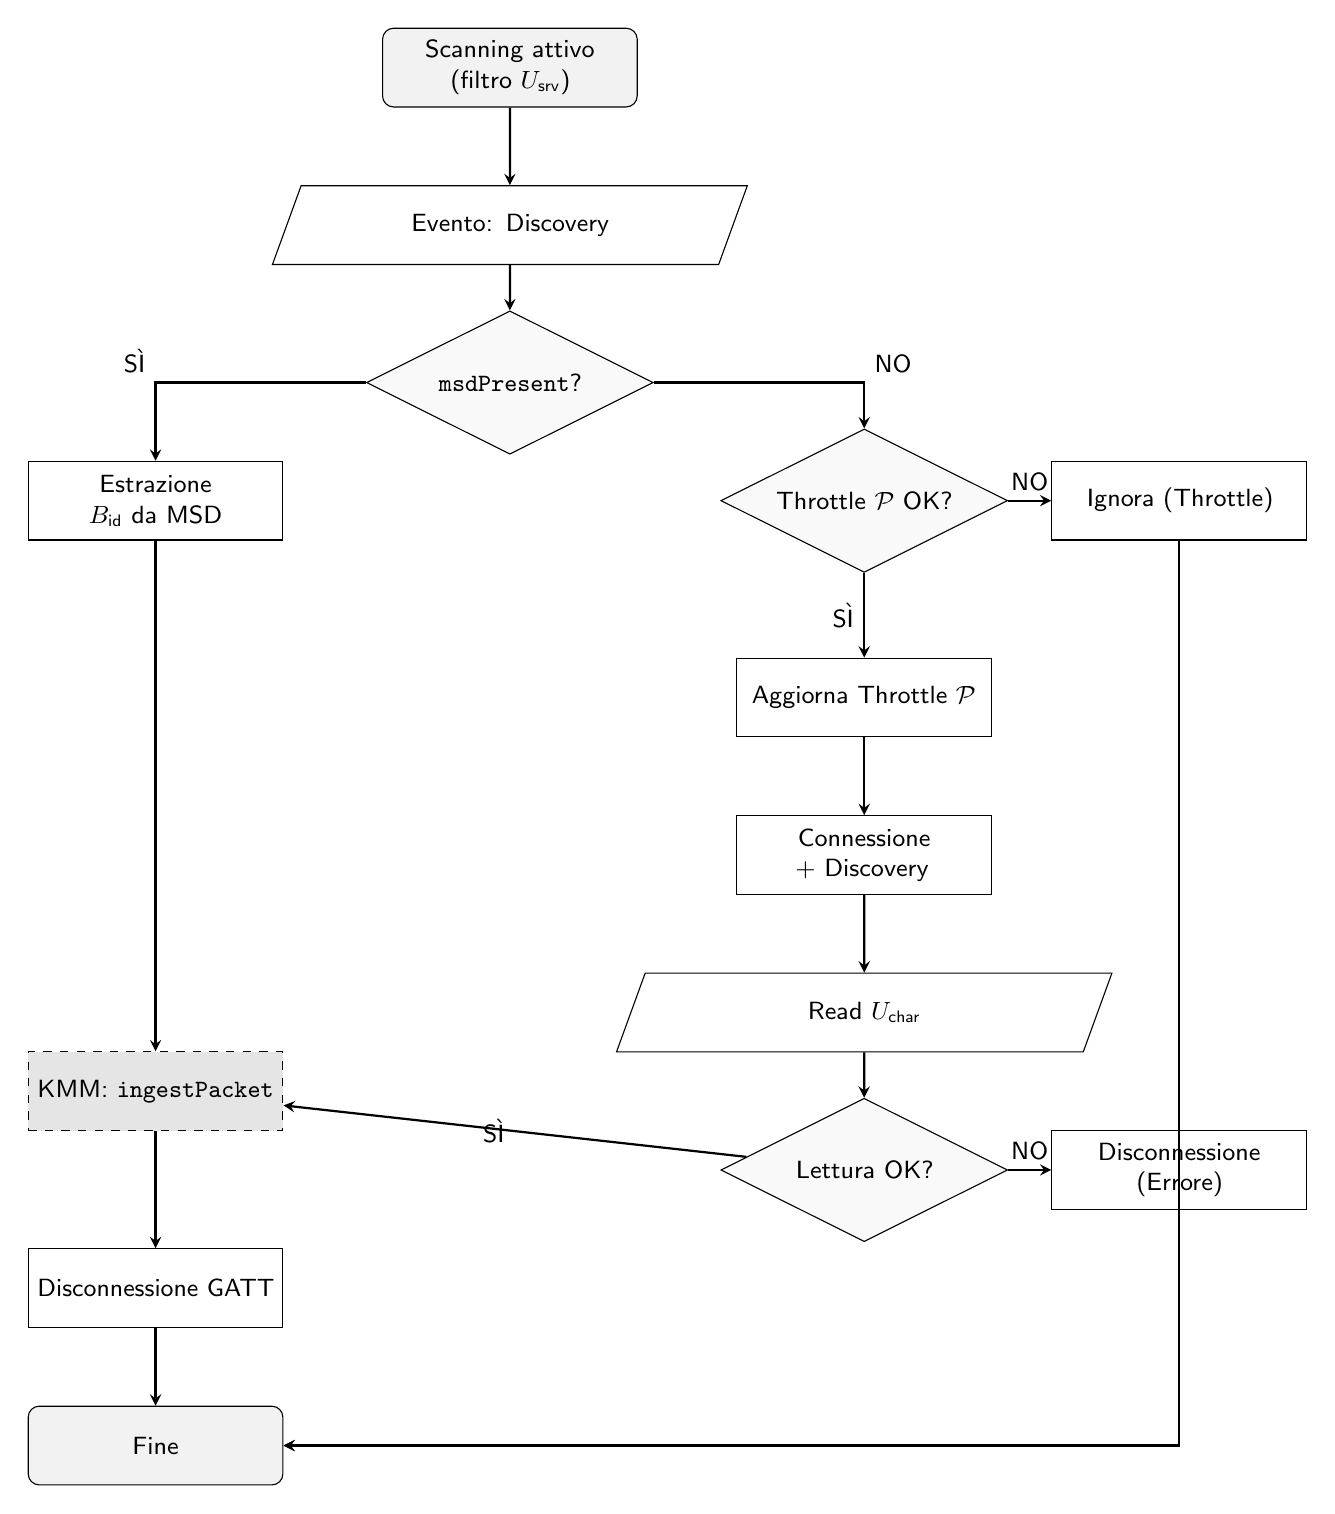
\begin{tikzpicture}[
            node distance=2cm,
            auto,
            font=\small\sffamily,
            % Larghezza fissa per evitare sforamento
            startstop/.style={rectangle, rounded corners, minimum width=3cm, minimum height=1cm, text centered, draw=black, fill=gray!10, text width=3cm},
            process/.style={rectangle, minimum width=3cm, minimum height=1cm, text centered, draw=black, fill=white, text width=3cm},
            decision/.style={diamond, aspect=2, minimum width=3cm, minimum height=1cm, text centered, draw=black, fill=gray!5, text width=2.5cm},
            kmm/.style={rectangle, minimum width=3cm, minimum height=1cm, text centered, draw=black, fill=gray!20, dashed, text width=3cm},
            arrow/.style={thick,->,>=stealth},
            io/.style={trapezium, trapezium left angle=70, trapezium right angle=110, minimum width=3cm, minimum height=1cm, text centered, draw=black, fill=white, text width=2.5cm}
        ]

        % Nodi
        \node (start) [startstop] {Scanning attivo (filtro \(U_{\text{srv}}\))};
        \node (discovery) [io, below of=start] {Evento: Discovery};

        \node (msd_check) [decision, below of=discovery] {\texttt{msdPresent}?};

        % Ramo GAP (SX) - Più stretto a sinistra
        \node (extract_msd) [process, left of=msd_check, xshift=-2.5cm, yshift=-1.5cm] {Estrazione \(B_{\text{id}}\) da MSD};

        % Ramo GATT (DX) - Più stretto a destra
        \node (throttle_check) [decision, right of=msd_check, xshift=2.5cm, yshift=-1.5cm] {Throttle \(\mathcal{P}\) OK?};

        % Nodo Ignora spostato sotto per risparmiare larghezza
        \node (ignore) [process, right of=throttle_check, xshift=2cm] {Ignora (Throttle)};

        \node (update_throttle) [process, below of=throttle_check, yshift=-0.5cm] {Aggiorna Throttle \(\mathcal{P}\)};
        \node (connect) [process, below of=update_throttle] {Connessione + Discovery};
        \node (read_gatt) [io, below of=connect] {Read \(U_{\text{char}}\)};
        \node (read_ok) [decision, below of=read_gatt] {Lettura OK?};

        % Errore spostato a destra ma stretto
        \node (disconnect_err) [process, right of=read_ok, xshift=2cm] {Disconnessione (Errore)};

        % Punto di convergenza Ingestione (Centrale sotto)
        \node (ingest) [kmm, below of=extract_msd, yshift=-5.5cm] {KMM: \texttt{ingestPacket}};

        % Disconnessione post-GATT
        \node (disconnect_ok) [process, below of=ingest, yshift=-0.5cm] {Disconnessione GATT};

        \node (end) [startstop, below of=disconnect_ok] {Fine};

        % Collegamenti
        \draw [arrow] (start) -- (discovery);
        \draw [arrow] (discovery) -- (msd_check);

        % Ramo GAP -> Ingest
        \draw [arrow] (msd_check) -| node[anchor=south east] {SÌ} (extract_msd);
        \draw [arrow] (extract_msd) -- (ingest);

        % Ramo GATT -> Throttle
        \draw [arrow] (msd_check) -| node[anchor=south west] {NO} (throttle_check);
        \draw [arrow] (throttle_check) -- node[anchor=south] {NO} (ignore);

        % Collegamento lungo per Ignora -> Fine
        \draw [arrow] (ignore) |- (end);

        % Ramo GATT -> Connessione
        \draw [arrow] (throttle_check) -- node[anchor=east] {SÌ} (update_throttle);
        \draw [arrow] (update_throttle) -- (connect);
        \draw [arrow] (connect) -- (read_gatt);
        \draw [arrow] (read_gatt) -- (read_ok);

        % Ramo GATT -> Errore Lettura
        \draw [arrow] (read_ok) -- node[anchor=south] {NO} (disconnect_err);
        \draw [arrow] (disconnect_err) |- (end);

        % Ramo GATT -> Ingest (Collega al nodo ingest centrale)
        \draw [arrow] (read_ok) -- node[anchor=east] {SÌ} (ingest);

        % Convergenza finale
        \draw [arrow] (ingest) -- (disconnect_ok);
        \draw [arrow] (disconnect_ok) -- (end);

    \end{tikzpicture}
    \caption{Flusso di Scanning ibrido e Ingestione}
    \label{fig:ios_scanning_flow}
\end{figure}

\section{Modulo Android (\texttt{:androidApp})}
Il modulo Android implementa la logica BLE nativa tramite lo stack \texttt{android.bluetooth.*}. Il controllo del flusso resta nativo: l’esecuzione è mantenuta continua tramite \texttt{BleService} (\emph{Foreground Service}) e tutte le invocazioni al modulo condiviso avvengono \emph{solo} tramite le procedure pubbliche di \texttt{Core} (KMM), preservando la semantica FIFO della coda persistente \(\mathcal{T}_{\text{queue}}\) e del batch \(\mathcal{T}_{\text{batch}}\) (definiti nello \emph{Strato Condiviso (KMM)}).

\subsection{\texttt{BleService}}
\texttt{BleService} è un \emph{Foreground Service} che possiede e coordina:
\begin{itemize}[nosep]
    \item \texttt{BluetoothLeAdvertiser} per advertising (ruolo \emph{peripheral});
    \item \texttt{BluetoothLeScanner} per scanning (ruolo \emph{central});
    \item \texttt{BluetoothGattServer} per server GATT quando la modalità locale richiede \(\text{GATT}\);
    \item lo scheduling (timer) delle invocazioni periodiche/event-driven verso KMM:
          \\ \texttt{Core.ensureAdvertisingBatch}, \texttt{Core.getCurrentBid}, \texttt{Core.ingestPacket}, \texttt{Core.syncQueue}.
\end{itemize}
Ogni transizione BLE e ogni invocazione KMM è serializzata su un’unica coda di esecuzione (single-queue), prevenendo interleaving non deterministici.

\subsubsection{Stato foreground/background e politica in background}
Si riusa \(\sigma \in \{\mathrm{FG},\mathrm{BG}\}\) come stato dell’applicazione (foreground/background), già introdotto nel documento.
In Android, \(\sigma\) è derivato dal lifecycle di processo (es. \emph{process in foreground} se esiste almeno una \texttt{Activity} in stato \texttt{RESUMED}; altrimenti \(\sigma=\mathrm{BG}\)).
\emph{Uso:} abilita la commutazione deterministica richiesta dalla matrice nel solo caso Android \(\mathrm{BG}\Rightarrow \text{GAP/GATT}\).

\textbf{Definizione (\(\rho\)):}
Sia
\[
    \rho \in \{\mathrm{GAP}, \mathrm{GATT}\}
\]
la politica configurabile di trasporto locale quando \(\sigma=\mathrm{BG}\).
\emph{Uso:} realizza la cella \emph{BG Android = GAP/GATT}: se \(\rho=\mathrm{GAP}\) si continua a trasmettere \(B_{\text{id}}\) in MSD anche in background; se \(\rho=\mathrm{GATT}\) si trasmette per discovery solo \(U_{\text{srv}}\) e si rende \(B_{\text{id}}\) leggibile via \(U_{\text{char}}\).
\emph{Origine (vincolante):} \(\rho\) è scelto dall’utente dalla UI tramite un controllo a scelta esclusiva con due soli valori: \(\mathrm{GAP}\) e \(\mathrm{GATT}\).
\emph{Persistenza (vincolante):} su Android il valore è salvato in \texttt{EncryptedSharedPreferences} con chiave \texttt{bg\_transport\_mode} e letto da \texttt{BleService} a ogni invocazione di \texttt{applyAdvertisingMode}.
\emph{Default (vincolante):} al primo avvio, se la chiave non esiste, vale \(\rho=\mathrm{GAP}\).


\subsubsection{Implementazione della matrice BLE}
Le costanti \(U_{\text{srv}}, U_{\text{char}}, C_{\text{id}}\) sono definite nella sezione \emph{Matrice di comportamento BLE}.

Si riusa il predicato \(\text{msdPresent}\) (già introdotto nel documento) come discriminante tra lettura diretta in \(\text{GAP}\) e fallback \(\text{GATT}\) in scanning.

\paragraph{Regola (Advertising Android):}
\begin{itemize}[nosep]
    \item se \(\sigma=\mathrm{FG}\), l’advertising è \(\text{GAP}\): il payload \(B_{\text{id}}\) è inserito in MSD;
    \item se \(\sigma=\mathrm{BG}\), allora:
          \begin{itemize}[nosep]
              \item se \(\rho=\mathrm{GAP}\), l’advertising resta \(\text{GAP}\) (MSD presente);
              \item se \(\rho=\mathrm{GATT}\), l’advertising è \(\text{GATT}\): l’advertisement contiene \(U_{\text{srv}}\) e \(B_{\text{id}}\) è leggibile via \(U_{\text{char}}\).
          \end{itemize}
\end{itemize}

\paragraph{Regola (Scanning Android):}
lo scanning è sempre filtrato su \(U_{\text{srv}}\). Per ogni peripheral scoperto:
\begin{itemize}[nosep]
    \item se \(\text{msdPresent}=\text{Vero}\), si acquisisce \(B_{\text{id}}\) in \(\text{GAP}\) e si invoca \(\texttt{Core.ingestPacket}\);
    \item se \(\text{msdPresent}=\text{Falso}\), si attiva fallback \(\text{GATT}\) e si legge \(U_{\text{char}}\) tramite \texttt{GattClientManager}.
\end{itemize}

\subsubsection{Precondizioni di piattaforma}
\texttt{BleService} applica una precondizione necessaria prima di attivare advertising/scanning:
\begin{itemize}[nosep]
    \item adapter Bluetooth disponibile e abilitato;
    \item supporto BLE e supporto advertising (device-dependent);
    \item permessi runtime coerenti con la versione Android:
          \begin{itemize}[nosep]
              \item Android \(\ge 12\): \texttt{BLUETOOTH\_SCAN}, \texttt{BLUETOOTH\_ADVERTISE}, \texttt{BLUETOOTH\_CONNECT};
              \item Android \(< 12\): permessi BLE + vincolo storico di location per scan (es. \texttt{ACCESS\_FINE\_LOCATION}).
          \end{itemize}
\end{itemize}
Se una precondizione non è soddisfatta, \texttt{BleService} impone \texttt{stopAdvertising} e \texttt{stopScan} e chiude eventuali sessioni GATT pendenti. Nessuna modifica su \(\mathcal{T}_{\text{batch}}\) o \(\mathcal{T}_{\text{queue}}\) avviene fuori da KMM.

\subsubsection{Inizializzazione e ripristino invarianti operative}
All’avvio del servizio (o quando lo stato Bluetooth torna utilizzabile), \texttt{BleService} ricostruisce in modo idempotente le invarianti:
\begin{itemize}[nosep]
    \item avvia scanning filtrato su \(U_{\text{srv}}\);
    \item riallinea l’advertising alla regola imposta da \((\sigma,\rho)\) tramite \texttt{applyAdvertisingMode} (definita sotto);
    \item attiva:
          \begin{itemize}[nosep]
              \item timer di bordo slot (riallineamento a \(S_{\text{slot}}\));
              \item timer periodico di periodo \(\tau\) per batch/coda.
          \end{itemize}
\end{itemize}
Le operazioni sono idempotenti: ripetizioni non producono effetti persistenti aggiuntivi, perché ogni side-effect su disco è mediato da KMM.

\subsubsection{Advertising e commutazione}
\texttt{BleService} non costruisce \(B_{\text{id}}\): richiede il payload a KMM tramite \texttt{Core.getCurrentBid} (definita nello \emph{Strato Condiviso (KMM)}).

\paragraph{Composizione MSD (solo modalità \(\text{GAP}\)):}
In \(\text{GAP}\) si usa la struttura MSD coerente con il documento:
\[
    D = C_{\text{id}} \ \| \ B_{\text{id}}.
\]
In Android, l’API separa l’header \(C_{\text{id}}\) dal payload: si configura il Company ID a valore \(C_{\text{id}}\) e si inseriscono i soli \(\SI{16}{\byte}\) di \(B_{\text{id}}\) come dati; la validazione \(\text{msdPresent}\) resta definita in modo equivalente perché l’\emph{AD structure} risultante contiene esattamente header + payload.

\paragraph{Procedura (\texttt{applyAdvertisingMode}):}
La procedura è invocata quando:
\begin{itemize}[nosep]
    \item le precondizioni BLE diventano vere (Bluetooth ON + permessi);
    \item \(\sigma\) cambia (FG\(\leftrightarrow\)BG);
    \item \(\rho\) cambia (solo se \(\sigma=\mathrm{BG}\));
    \item cambia lo slot temporale \(S_{\text{slot}}\) (timer di slot).
\end{itemize}
I passi sono:
\begin{enumerate}
    \item invocare \texttt{Core.ensureAdvertisingBatch()} per garantire copertura del batch in condizioni di rete;
    \item richiedere \(b \leftarrow \texttt{Core.getCurrentBid}()\);
    \item se \(b=\texttt{null}\), eseguire:
          \[
              \texttt{stopAdvertising}
          \]
          e, se un server GATT era attivo per trasporto locale \(\text{GATT}\), lasciarlo pubblicato ma rispondere alle read con errore (sezione \emph{Server GATT});
    \item se \(b\neq \texttt{null}\), determinare la modalità locale:
          \[
              \mu =
              \begin{cases}
                  \mathrm{GAP} & \text{se }\sigma=\mathrm{FG} \\
                  \rho         & \text{se }\sigma=\mathrm{BG}
              \end{cases}
          \]
          e applicare:
          \begin{itemize}[nosep]
              \item se \(\mu=\mathrm{GAP}\): \texttt{stopAdvertising} \(\rightarrow\) \texttt{startAdvertising} includendo \(U_{\text{srv}}\) e MSD con \(b\);
              \item se \(\mu=\mathrm{GATT}\): \texttt{stopAdvertising} \(\rightarrow\) \texttt{ensureGattServerPublished} (servizio \(U_{\text{srv}}\) + caratteristica \(U_{\text{char}}\)) \(\rightarrow\) \texttt{startAdvertising} includendo \(U_{\text{srv}}\) (nessun MSD).
          \end{itemize}
\end{enumerate}
La procedura è idempotente: invocazioni ripetute producono uno stato BLE equivalente, a parità di \((\sigma,\rho)\) e di \(b\).

\subsubsection{Timer di slot}
Si riusano \(t_{\text{unix}}, \Delta t_{\text{slot}}, S_{\text{slot}}\) definiti nello \emph{Strato Condiviso (KMM)}.

Dato \(t_{\text{unix}}\), \texttt{BleService} programma un timer a singola scadenza sul bordo successivo:
\[
    t_{\text{next}} = (S_{\text{slot}} + 1)\cdot \Delta t_{\text{slot}}.
\]
Alla scadenza, invoca \texttt{applyAdvertisingMode} e riprogramma sul bordo successivo. Questo garantisce assenza di drift: l’aggiornamento è ancorato ai bordi di slot, non a un periodo accumulativo.

\subsubsection{Server GATT}
Quando la modalità locale è \(\mathrm{GATT}\), \texttt{BleService} espone un server GATT che permette la lettura di \(B_{\text{id}}\) tramite \(U_{\text{char}}\).

\paragraph{Pubblicazione:}
\begin{itemize}[nosep]
    \item servizio con UUID \(U_{\text{srv}}\);
    \item caratteristica leggibile con UUID \(U_{\text{char}}\).
\end{itemize}

\paragraph{Semantica di read su \(U_{\text{char}}\):}
Alla richiesta di lettura, \texttt{BleService} risponde con:
\[
    b \leftarrow \texttt{Core.getCurrentBid}().
\]
Se \(b\neq\texttt{null}\), restituisce i \(\SI{16}{\byte}\) del payload; se \(b=\texttt{null}\), risponde con errore GATT (dato non disponibile). La correttezza temporale è garantita perché \(b\) è valutato al tempo della read (coerente con \(S_{\text{slot}}\) corrente).

\subsubsection{Scanning e ingestione \(\mathrm{GAP}\)}
Lo scanning è sempre filtrato per \(U_{\text{srv}}\).
Alla discovery di un peripheral:
\begin{enumerate}
    \item se \(\text{msdPresent}=\text{Vero}\), si estrae \(B_{\text{id}}\in\{0,1\}^{128}\) e si invoca immediatamente
          \[
              \texttt{Core.ingestPacket}(B_{\text{id}});
          \]
    \item se \(\text{msdPresent}=\text{Falso}\), si attiva fallback \(\mathrm{GATT}\) (sezione \texttt{GattClientManager}).
\end{enumerate}
La deduplica volatile e l’eventuale enqueue persistente sono interamente responsabilità di \texttt{Core.ingestPacket} (KMM).

\subsubsection{Scheduling invocazioni KMM}
Oltre al timer di slot, \texttt{BleService} programma un timer periodico \emph{best-effort} di periodo \(\tau\) (definito nello \emph{Strato Condiviso (KMM)}). A ogni tick invoca in ordine:
\begin{enumerate}
    \item \texttt{Core.ensureAdvertisingBatch()};
    \item \texttt{Core.syncQueue()}.
\end{enumerate}
Queste invocazioni preservano gli invarianti:
\begin{itemize}[nosep]
    \item se \texttt{ensureAdvertisingBatch} fallisce (rete/errore), \(\mathcal{T}_{\text{batch}}\) resta invariata;
    \item se \texttt{syncQueue} fallisce (rete/risposta non valida), \(\mathcal{T}_{\text{queue}}\) resta invariata e la FIFO è preservata;
    \item la semantica \(1{:}1\) è garantita da \texttt{Core.syncQueue} (al più un elemento per tick).
\end{itemize}

\subsubsection{Trigger evento-driven}
Oltre ai timer, \texttt{BleService} invoca KMM in punti deterministici:
\begin{itemize}[nosep]
    \item su soddisfazione precondizioni BLE (BT ON + permessi): \texttt{applyAdvertisingMode} e avvio scanning;
    \item su cambio \(\sigma\) o \(\rho\): \texttt{applyAdvertisingMode} (commuta deterministica GAP\(\leftrightarrow\)GATT quando richiesto);
    \item su acquisizione payload (GAP o GATT): invocazione immediata \texttt{Core.ingestPacket};
    \item su errore di advertising/scanning (callback di failure o stop imposto dal sistema): riapplicazione idempotente del pipeline via \texttt{applyAdvertisingMode} e restart scanning quando le precondizioni tornano valide.
\end{itemize}

\subsection{\texttt{GattClientManager}}
\texttt{GattClientManager} implementa la sequenza di connessione e read necessaria quando lo scanner rileva \(U_{\text{srv}}\) ma \(\text{msdPresent}=\text{Falso}\) (caso tipico: trasmittente iOS in BG, oppure Android in BG con \(\rho=\mathrm{GATT}\)).

Si riusano \(\iota\) (identificatore opaco di peripheral) e \(\mathcal{P}\) (cache volatile per throttle dei tentativi GATT) già introdotti nel documento, così come \(\tau\) (finestra minima tra tentativi).

\subsubsection{Regola}
Un tentativo GATT verso \(\iota\) è ammesso se e solo se:
\[
    \neg \exists(\iota,t)\in\mathcal{P}\ \mid\ (t_{\text{unix}}-t)<\tau.
\]
All’avvio del tentativo, \(\mathcal{P}\) viene aggiornata sostituendo l’eventuale coppia per \(\iota\) con \((\iota,t_{\text{unix}})\). Tale aggiornamento, eseguito all’inizio, impedisce connessioni duplicate concorrenti verso lo stesso \(\iota\) (ogni nuovo tentativo cadrebbe nella finestra \(\tau\)).

\subsubsection{Procedura}
Dato un peripheral \(\iota\) eleggibile:
\begin{enumerate}
    \item connessione GATT (\texttt{connectGatt} con \texttt{autoConnect} disabilitato);
    \item discovery servizi, selezione del servizio \(U_{\text{srv}}\);
    \item discovery/lookup della caratteristica \(U_{\text{char}}\);
    \item read \texttt{readCharacteristic} su \(U_{\text{char}}\);
    \item se la lettura produce un valore \(B_{\text{id}}\in\{0,1\}^{128}\), invocazione
          \[
              \texttt{Core.ingestPacket}(B_{\text{id}});
          \]
    \item disconnessione e rilascio risorse (\texttt{disconnect} e \texttt{close}) per evitare leak di sessioni.
\end{enumerate}

\subsubsection{Gestione errori e timeout}
Qualunque fallimento tecnico (connessione, discovery, read) termina la procedura senza invocare \texttt{Core.ingestPacket}. La sessione viene chiusa e il peripheral resta soggetto alla regola di throttle tramite \(\mathcal{P}\).
Un tentativo che non completa entro una finestra massima coerente con la politica di throttle viene abortito con disconnessione esplicita; la scelta della finestra massima è vincolata a essere finita e non superiore, per ordine di grandezza, alla scala temporale già usata per evitare retry aggressivi (cioè \(\tau\)).

\subsection{Flussi di Esecuzione Android}
Di seguito sono riportati i diagrammi di flusso che illustrano le principali logiche decisionali e operative del modulo Android, riflettendo la gestione tramite \emph{Foreground Service} e timer locali.

\subsubsection{Ciclo di Vita e Gestione Stato}
Questo diagramma mostra come \texttt{BleService} gestisce l'avvio, le precondizioni (Bluetooth/Permessi) e la determinazione della modalità operativa locale basata sullo stato del processo (\(\sigma\)) e sulla configurazione utente (\(\rho\)).

\begin{figure}[H]
    \centering
    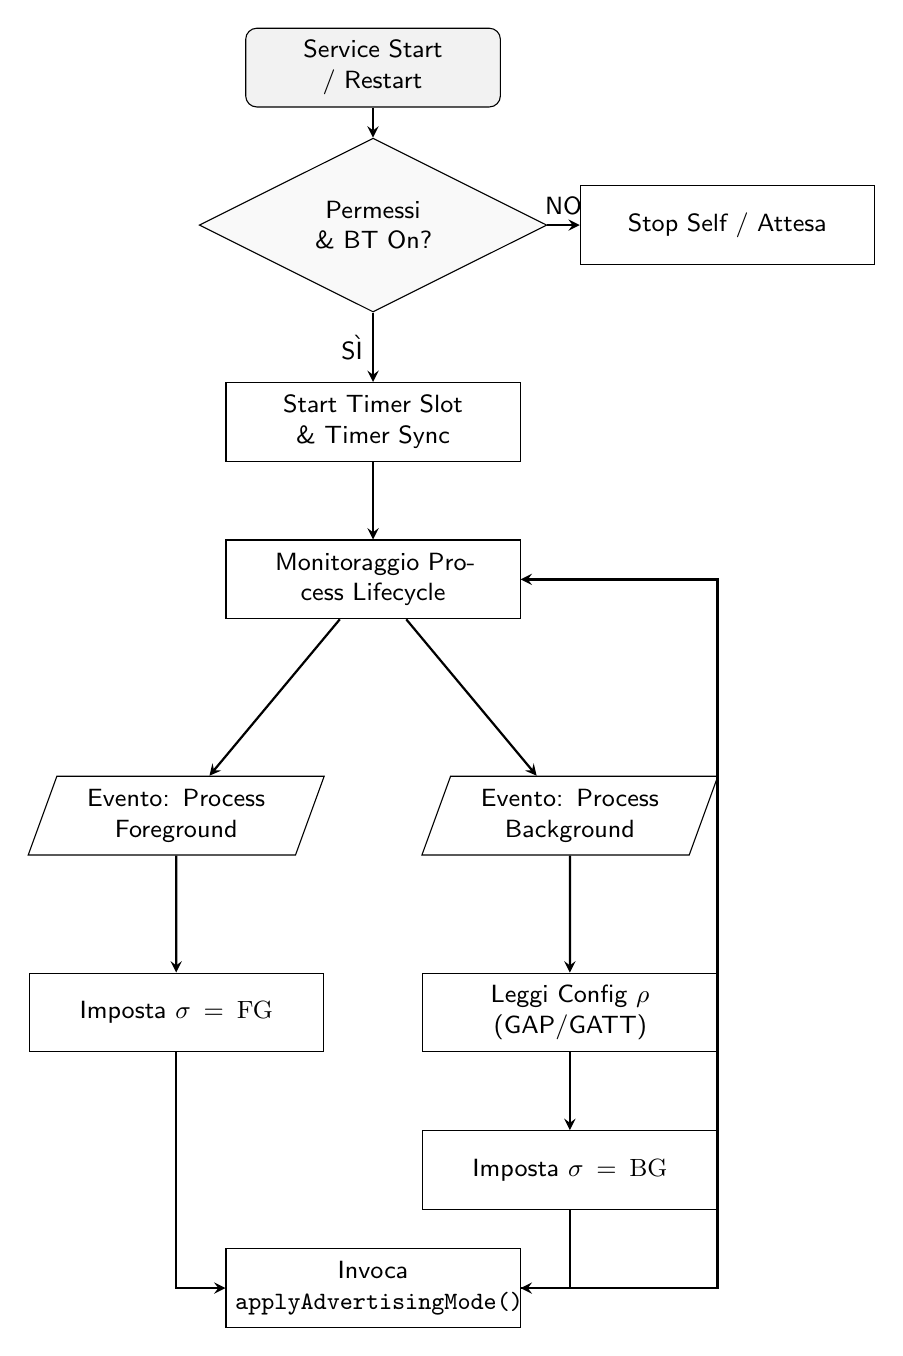
\begin{tikzpicture}[
            node distance=2cm,
            auto,
            font=\small\sffamily,
            % Stili con larghezza fissa
            startstop/.style={rectangle, rounded corners, minimum width=3cm, minimum height=1cm, text centered, draw=black, fill=gray!10, text width=3cm},
            process/.style={rectangle, minimum width=3.5cm, minimum height=1cm, text centered, draw=black, fill=white, text width=3.5cm},
            decision/.style={diamond, aspect=2, minimum width=3cm, minimum height=1cm, text centered, draw=black, fill=gray!5, text width=2.5cm},
            arrow/.style={thick,->,>=stealth},
            io/.style={trapezium, trapezium left angle=70, trapezium right angle=110, minimum width=3.5cm, minimum height=1cm, text centered, draw=black, fill=white, text width=2.5cm}
        ]

        % Nodi
        \node (start) [startstop] {Service Start / Restart};
        \node (perm_check) [decision, below of=start] {Permessi \& BT On?};

        \node (stop_self) [process, right of=perm_check, xshift=2.5cm] {Stop Self / Attesa};

        \node (init_timers) [process, below of=perm_check, yshift=-0.5cm] {Start Timer Slot \& Timer Sync};

        \node (lifecycle_mon) [process, below of=init_timers] {Monitoraggio Process Lifecycle};

        % Eventi
        \node (event_fg) [io, below of=lifecycle_mon, xshift=-2.5cm, yshift=-1cm] {Evento: Process Foreground};
        \node (event_bg) [io, below of=lifecycle_mon, xshift=2.5cm, yshift=-1cm] {Evento: Process Background};

        \node (set_fg) [process, below of=event_fg, yshift=-0.5cm] {Imposta \(\sigma = \mathrm{FG}\)};

        % Gestione Configurazione Rho per BG
        \node (read_rho) [process, below of=event_bg, yshift=-0.5cm] {Leggi Config \(\rho\) (GAP/GATT)};
        \node (set_bg) [process, below of=read_rho] {Imposta \(\sigma = \mathrm{BG}\)};

        % Nodo centrale convergenza
        \node (apply_mode) [process, below of=lifecycle_mon, yshift=-7cm] {Invoca \texttt{applyAdvertisingMode()}};

        % Collegamenti
        \draw [arrow] (start) -- (perm_check);
        \draw [arrow] (perm_check) -- node[anchor=south] {NO} (stop_self);
        \draw [arrow] (perm_check) -- node[anchor=east] {SÌ} (init_timers);

        \draw [arrow] (init_timers) -- (lifecycle_mon);

        \draw [arrow] (lifecycle_mon) -- (event_fg);
        \draw [arrow] (lifecycle_mon) -- (event_bg);

        \draw [arrow] (event_fg) -- (set_fg);
        \draw [arrow] (event_bg) -- (read_rho);
        \draw [arrow] (read_rho) -- (set_bg);

        \draw [arrow] (set_fg) |- (apply_mode);
        \draw [arrow] (set_bg) |- (apply_mode);

        % Loop ritorno
        \draw [arrow] (apply_mode.east) -- ++(2.5cm,0) |- (lifecycle_mon.east);

    \end{tikzpicture}
    \caption{Flusso Android: Ciclo di vita e aggiornamento stato}
    \label{fig:android_lifecycle_flow}
\end{figure}

\newpage

\subsubsection{Logica di Advertising}
Questo diagramma dettaglia la procedura \texttt{applyAdvertisingMode}. Evidenzia la gestione idempotente e la selezione della modalità di trasporto (\(\mu\)) in base alla combinazione di \(\sigma\) e \(\rho\), interagendo con il KMM per ottenere il payload.

\begin{figure}[H]
    \centering
    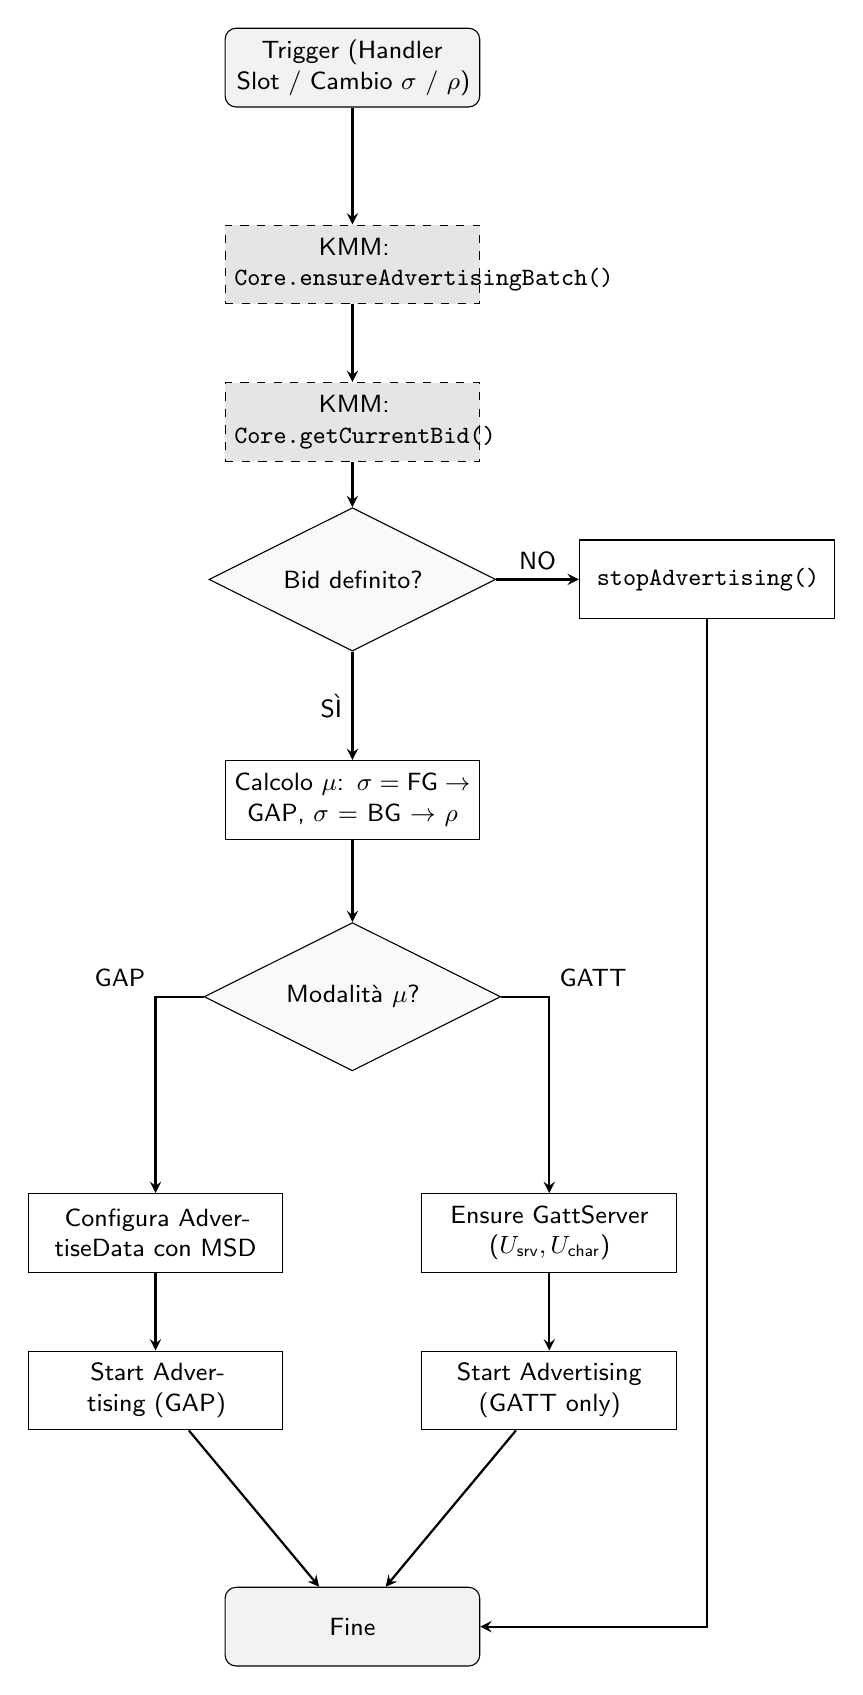
\begin{tikzpicture}[
            node distance=2cm,
            auto,
            font=\small\sffamily,
            startstop/.style={rectangle, rounded corners, minimum width=3cm, minimum height=1cm, text centered, draw=black, fill=gray!10, text width=3cm},
            process/.style={rectangle, minimum width=3cm, minimum height=1cm, text centered, draw=black, fill=white, text width=3cm},
            decision/.style={diamond, aspect=2, minimum width=3cm, minimum height=1cm, text centered, draw=black, fill=gray!5, text width=2.5cm},
            kmm/.style={rectangle, minimum width=3cm, minimum height=1cm, text centered, draw=black, fill=gray!20, dashed, text width=3cm},
            arrow/.style={thick,->,>=stealth}
        ]

        % Nodi
        \node (start) [startstop] {Trigger (Handler Slot / Cambio \(\sigma\) / \(\rho\))};

        \node (ensure_batch) [kmm, below of=start, yshift=-0.5cm] {KMM: \texttt{Core.ensureAdvertisingBatch()}};
        \node (get_bid) [kmm, below of=ensure_batch] {KMM: \texttt{Core.getCurrentBid()}};
        \node (bid_check) [decision, below of=get_bid] {Bid definito?};

        \node (stop_ad) [process, right of=bid_check, xshift=2.5cm] {\texttt{stopAdvertising()}};

        \node (mode_calc) [process, below of=bid_check, yshift=-0.8cm] {Calcolo \(\mu\): \(\sigma=\text{FG} \to \text{GAP}\), \(\sigma=\text{BG} \to \rho\)};
        \node (mu_check) [decision, below of=mode_calc, yshift=-0.5cm] {Modalità \(\mu\)?};

        % Ramo GAP (SX)
        \node (gap_conf) [process, below of=mu_check, xshift=-2.5cm, yshift=-1cm] {Configura AdvertiseData con MSD};
        \node (gap_start) [process, below of=gap_conf] {Start Advertising (GAP)};

        % Ramo GATT (DX)
        \node (gatt_server) [process, below of=mu_check, xshift=2.5cm, yshift=-1cm] {Ensure GattServer (\(U_{\text{srv}}, U_{\text{char}}\))};
        \node (gatt_start) [process, below of=gatt_server] {Start Advertising (GATT only)};

        \node (end) [startstop, below of=mu_check, yshift=-6cm] {Fine};

        % Collegamenti
        \draw [arrow] (start) -- (ensure_batch);
        \draw [arrow] (ensure_batch) -- (get_bid);
        \draw [arrow] (get_bid) -- (bid_check);

        \draw [arrow] (bid_check) -- node[anchor=south] {NO} (stop_ad);
        \draw [arrow] (stop_ad) |- (end);

        \draw [arrow] (bid_check) -- node[anchor=east] {SÌ} (mode_calc);
        \draw [arrow] (mode_calc) -- (mu_check);

        \draw [arrow] (mu_check) -| node[anchor=south east] {GAP} (gap_conf);
        \draw [arrow] (gap_conf) -- (gap_start);
        \draw [arrow] (gap_start) -- (end);

        \draw [arrow] (mu_check) -| node[anchor=south west] {GATT} (gatt_server);
        \draw [arrow] (gatt_server) -- (gatt_start);
        \draw [arrow] (gatt_start) -- (end);

    \end{tikzpicture}
    \caption{Flusso decisione Advertising Android (\(\mu\))}
    \label{fig:android_advertising_flow}
\end{figure}

\newpage

\subsubsection{Scanning e Fallback GATT}
Questo diagramma illustra la logica di ricezione nel \texttt{BleService} e la delega al \texttt{GattClientManager}. Mostra il check MSD, il throttle locale per le connessioni e l'uso finale di \texttt{Core.ingestPacket}.

\begin{figure}[H]
    \centering
    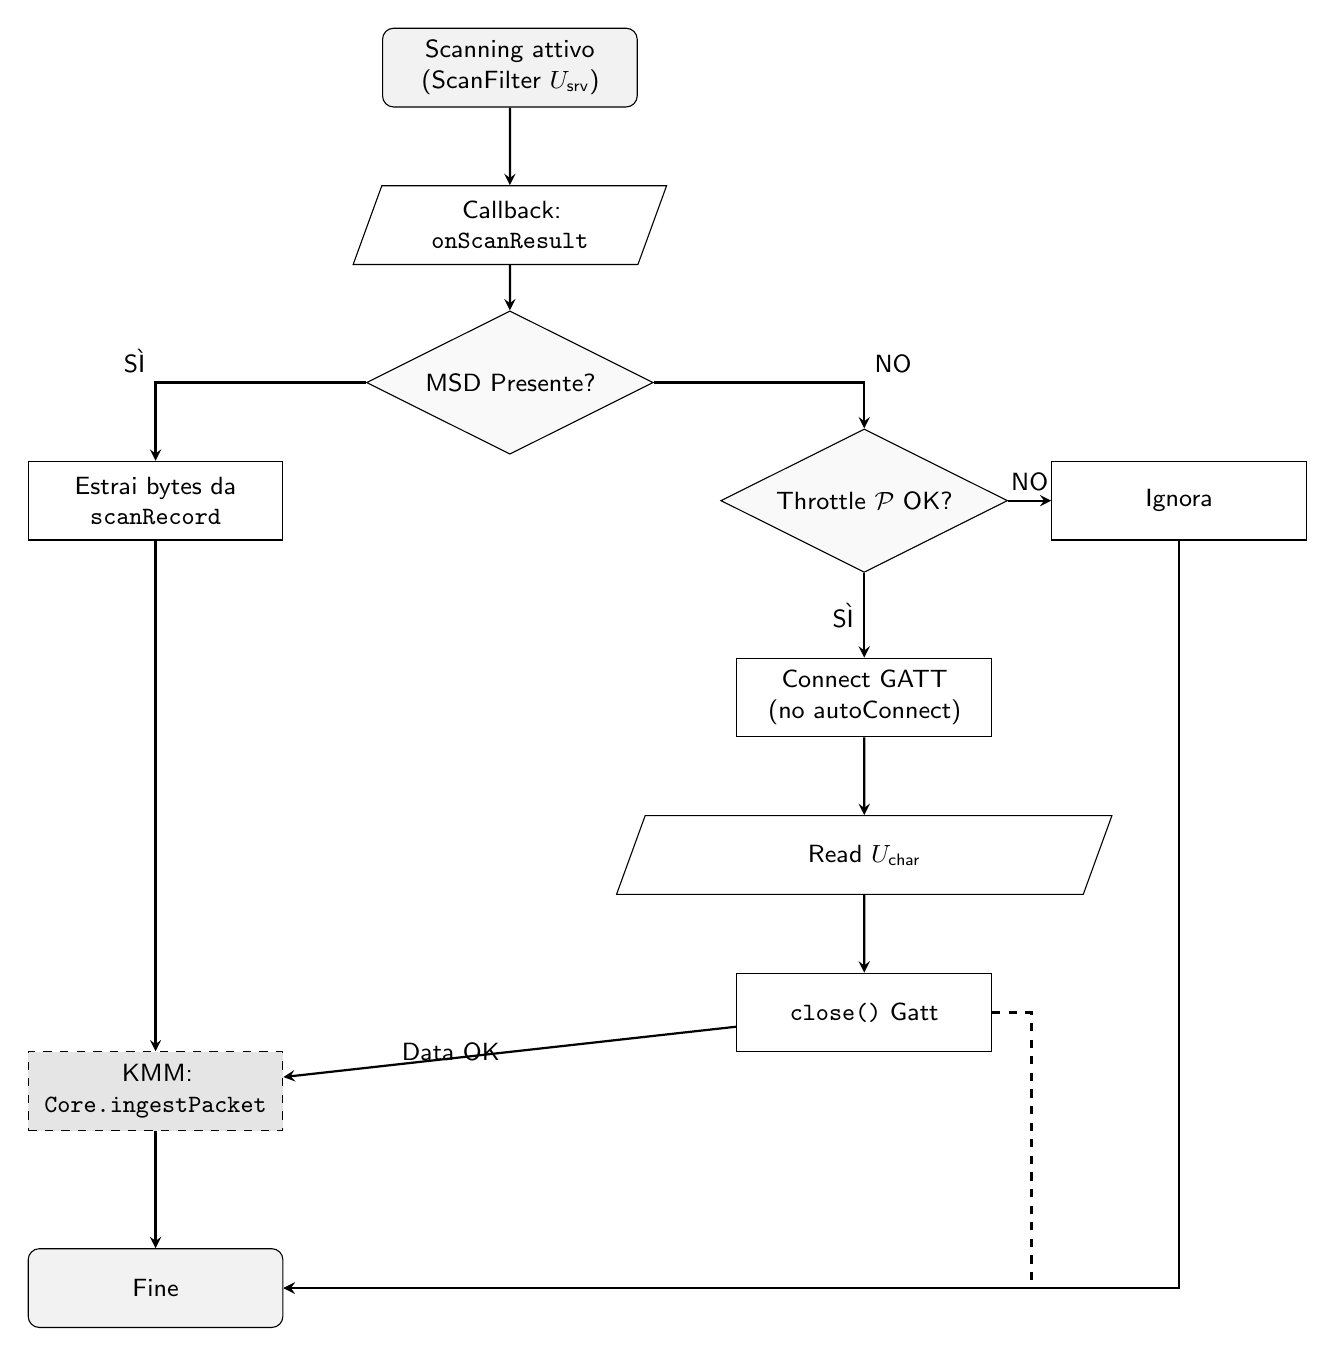
\begin{tikzpicture}[
            node distance=2cm,
            auto,
            font=\small\sffamily,
            startstop/.style={rectangle, rounded corners, minimum width=3cm, minimum height=1cm, text centered, draw=black, fill=gray!10, text width=3cm},
            process/.style={rectangle, minimum width=3cm, minimum height=1cm, text centered, draw=black, fill=white, text width=3cm},
            decision/.style={diamond, aspect=2, minimum width=3cm, minimum height=1cm, text centered, draw=black, fill=gray!5, text width=2.5cm},
            kmm/.style={rectangle, minimum width=3cm, minimum height=1cm, text centered, draw=black, fill=gray!20, dashed, text width=3cm},
            arrow/.style={thick,->,>=stealth},
            io/.style={trapezium, trapezium left angle=70, trapezium right angle=110, minimum width=3cm, minimum height=1cm, text centered, draw=black, fill=white, text width=2.5cm}
        ]

        % Nodi
        \node (start) [startstop] {Scanning attivo (ScanFilter \(U_{\text{srv}}\))};
        \node (callback) [io, below of=start] {Callback: \texttt{onScanResult}};

        \node (msd_check) [decision, below of=callback] {MSD Presente?};

        % Ramo GAP (SX)
        \node (extract) [process, left of=msd_check, xshift=-2.5cm, yshift=-1.5cm] {Estrai bytes da \texttt{scanRecord}};

        % Ramo GATT (DX) - Gestito da GattClientManager
        \node (throttle) [decision, right of=msd_check, xshift=2.5cm, yshift=-1.5cm] {Throttle \(\mathcal{P}\) OK?};
        \node (ignore) [process, right of=throttle, xshift=2cm] {Ignora};

        \node (connect) [process, below of=throttle, yshift=-0.5cm] {Connect GATT (no autoConnect)};
        \node (read) [io, below of=connect] {Read \(U_{\text{char}}\)};
        \node (close) [process, below of=read] {\texttt{close()} Gatt};

        % Convergenza Ingestione
        \node (ingest) [kmm, below of=extract, yshift=-5.5cm] {KMM: \texttt{Core.ingestPacket}};

        \node (end) [startstop, below of=ingest, yshift=-0.5cm] {Fine};

        % Collegamenti
        \draw [arrow] (start) -- (callback);
        \draw [arrow] (callback) -- (msd_check);

        % Ramo GAP
        \draw [arrow] (msd_check) -| node[anchor=south east] {SÌ} (extract);
        \draw [arrow] (extract) -- (ingest);

        % Ramo GATT
        \draw [arrow] (msd_check) -| node[anchor=south west] {NO} (throttle);

        \draw [arrow] (throttle) -- node[anchor=south] {NO} (ignore);
        \draw [arrow] (ignore) |- (end);

        \draw [arrow] (throttle) -- node[anchor=east] {SÌ} (connect);
        \draw [arrow] (connect) -- (read);
        \draw [arrow] (read) -- (close);

        % Ramo GATT -> Ingest (se lettura ok)
        \draw [arrow] (close) -- node[anchor=east] {Data OK} (ingest);

        % Errore GATT (implicito nel diagramma per brevità: va a Fine)
        \draw [arrow, dashed] (close.east) -- ++(0.5cm,0) |- (end.east);

        % Finale
        \draw [arrow] (ingest) -- (end);

    \end{tikzpicture}
    \caption{Flusso Android: Scanning GAP e Fallback GATT}
    \label{fig:android_scanning_flow}
\end{figure}

\end{document}